
%%
%% Copyright 2007, 2008, 2009 Elsevier Ltd
%%
%% This file is part of the 'Elsarticle Bundle'.
%% ---------------------------------------------
%%
%% It may be distributed under the conditions of the LaTeX Project Public
%% License, either version 1.2 of this license or (at your option) any
%% later version.  The latest version of this license is in
%%    http://www.latex-project.org/lppl.txt
%% and version 1.2 or later is part of all distributions of LaTeX
%% version 1999/12/01 or later.
%%
%% The list of all files belonging to the 'Elsarticle Bundle' is
%% given in the file `manifest.txt'.
%%

%% Template article for Elsevier's document class `elsarticle'
%% with numbered style bibliographic references
%% SP 2008/03/01
%%
%%
%%
%% $Id: elsarticle-template-num.tex 4 2009-10-24 08:22:58Z rishi $
%%
%%
\documentclass[preprint,12pt]{elsarticle}

%% Use the option review to obtain double line spacing
%% \documentclass[preprint,review,12pt]{elsarticle}

%% Use the options 1p,twocolumn; 3p; 3p,twocolumn; 5p; or 5p,twocolumn
%% for a journal layout:
%% \documentclass[final,1p,times]{elsarticle}
%% \documentclass[final,1p,times,twocolumn]{elsarticle}
%% \documentclass[final,3p,times]{elsarticle}
%% \documentclass[final,3p,times,twocolumn]{elsarticle}
%% \documentclass[final,5p,times]{elsarticle}
%% \documentclass[final,5p,times,twocolumn]{elsarticle}

%% if you use PostScript figures in your article
%% use the graphics package for simple commands
%% \usepackage{graphics}
%% or use the graphicx package for more complicated commands
%% \usepackage{graphicx}
%% or use the epsfig package if you prefer to use the old commands
%% \usepackage{epsfig}

%% The amssymb package provides various useful mathematical symbols
\usepackage{amssymb}
%% The amsthm package provides extended theorem environments
%% \usepackage{amsthm}

%% The lineno packages adds line numbers. Start line numbering with
%% \begin{linenumbers}, end it with \end{linenumbers}. Or switch it on
%% for the whole article with \linenumbers after \end{frontmatter}.
%% \usepackage{lineno}

%% natbib.sty is loaded by default. However, natbib options can be
%% provided with \biboptions{...} command. Following options are
%% valid:

%%   round  -  round parentheses are used (default)
%%   square -  square brackets are used   [option]
%%   curly  -  curly braces are used      {option}
%%   angle  -  angle brackets are used    <option>
%%   semicolon  -  multiple citations separated by semi-colon
%%   colon  - same as semicolon, an earlier confusion
%%   comma  -  separated by comma
%%   numbers-  selects numerical citations
%%   super  -  numerical citations as superscripts
%%   sort   -  sorts multiple citations according to order in ref. list
%%   sort&compress   -  like sort, but also compresses numerical citations
%%   compress - compresses without sorting
%%
%% \biboptions{comma,round}

% \biboptions{}

\usepackage{subfigure}
\usepackage{wrapfig}

\providecommand{\abs}[1]{\vert#1\vert}

\journal{Future Generation Computer Systems}

% For defining whether this is a paper or a report... 
\newcommand{\doctype}{paper} 
   
\begin{document}

\begin{frontmatter}

%% Title, authors and addresses

%% use the tnoteref command within \title for footnotes;
%% use the tnotetext command for the associated footnote;
%% use the fnref command within \author or \address for footnotes;
%% use the fntext command for the associated footnote;
%% use the corref command within \author for corresponding author footnotes;
%% use the cortext command for the associated footnote;
%% use the ead command for the email address,
%% and the form \ead[url] for the home page:
%%
%% \title{Title\tnoteref{label1}}
%% \tnotetext[label1]{}
%% \author{Name\corref{cor1}\fnref{label2}}
%% \ead{email address}
%% \ead[url]{home page}
%% \fntext[label2]{}
%% \cortext[cor1]{}
%% \address{Address\fnref{label3}}
%% \fntext[label3]{}

%\title{The mDNS Compatible INDI Service Discovery System}
\title{DNS Messaging for Service Discovery in Infrastructureless Mobile Networks}

%% use optional labels to link authors explicitly to addresses:
%% \author[label1,label2]{<author name>}
%% \address[label1]{<address>}
%% \address[label2]{<address>}

\author[nrl]{Joe Macker}

\author[cu]{Ian Taylor}

\address[nrl]{Naval Research Lab, Washington DC, USA}
\address[cu]{School of Computer Science, Cardiff University, Cardiff, UK}

\begin{abstract}
\sloppypar Service discovery is an important aspect of any automated distributed system and the more transient the distributed system's entities, the more problematic is this task.  In mobile ad-hoc networks (MANETs), where self-configuring infrastructureless networks of mobile devices are often connected by multi-hop wireless links, the challenge becomes significant with incongruous tradeoffs between state maintenance for reliability and bandwidth consumption for efficiency.  Potential solutions require techniques that can efficiently map the distributed application across a complexity of variable mobility patterns and underlying routing algorithms.  Existing standardized solutions for service discovery, such as mDNS, are inadequate because they employ a rather fixed set of timers that cannot adapt to different application scenarios and dynamics of the underlying network connectivity.   In this paper, we explore a combinatory approach that, on the one hand, leverages existing standardized service discovery messaging to ensure interoperability with mDNS and DNS, and then on the other,  provides flexible tuning of distributed modes of operation to serve the application's needs for a particular type of network. We discuss the application usages of such an approach and describe how these techniques can provide a bridging infrastructure for interoperability between mobile and fixed network infrastructures.  We show that by using this flexibility of tuning modes, we can create a proactive approach to service discovery, which we hypothesise can exhibit considerable efficiency and success rate gains over conventional techniques in transient mobile environments. We empirically prove this hypothesis by presenting results based on 96 different scenarios recorded using emulations representing real-world experiments that compare this approach with mDNS.      

\end{abstract}

\begin{keyword} mDNS \sep JmDNS \sep Peer-to-Peer \sep Multicast \sep Service Discovery \end{keyword}

%% keywords here, in the form: keyword \sep keyword

%% MSC codes here, in the form: \MSC code \sep code
%% or \MSC[2008] code \sep code (2000 is the default)

\end{frontmatter}

\section{Introduction} 
\label{sec:introduction} 
The emergence of Apple's Rendezvous for (now Bonjour) upon switching from SLP \cite{slp} with the launch of Mac OS X 10.2 ``Jaguar'' in August 2002, initiated a number of activities for standardization of a zero configuration protocol called Multicast Domain Name Service (mDNS, \cite{giordano2005dns,zeroconfbook}). Since then, mDNS has since gained probably the most widespread deployment across platforms of all of its predecessors.   Other systems, such as  the Service Location Protocol version 2 (SLPv2) \cite{guttman1999service} and the Simple Service Discovery Protocol (SSDP) in Microsoft's Universal Plug n' Play (UPnP) standard \cite{helal2002standards} are in use but have not gained quite as much impact.  

For wide area networks, service discovery has taken a somewhat simplified or application-specific  approach. Middleware systems such as  JINI \cite{jini} and Jxta \cite{Jxta} and SOA-based architectures such as UDDI directories \cite{uddi}, are based on simple mechanisms, supporting only basic multicast and/or unicast primitives for connecting to lookup servers, rendezvous nodes, and so forth. Most other service discovery in this space, even for the highly distributed peer-to-peer variety, tend to function at an application specific level once a node has connected to the application overlay using TCP, e.g. Limewire \cite{limewire} and Gnutella \cite{gnutella}.  The connection to the network itself e.g., the discovery of a ``Limewire peer'', is typically achieved through a centralized server list of good candidates. Although distributed query overlays (using rendezvous nodes) and distributed hash tables (DHTs, e.g. \cite{Ratnasamy01ascalable}) take different approaches, they also tend to be application specific by partitioning the network into sub-areas based on application-specific criteria and content e.g. file content, namespaces and cryptography keys, and so on.  


A similar approach through the use of a unicast connection is taken by mDNS to connect to the WAN, however, this has the added advantage that it leverages existing infrastructure for connecting a mDNS responder to a deployed DNS server. Since DNS is already ubiquitous on the Internet, programmers are already familiar with its interfaces and can deploy service advertisements using the same data structures that DNS does for other records.  In terms of uptake, dynamic discovery on a LAN and interoperability with existing infrastructure on a WAN therefore, it can be agued that mDNS seems to be gaining traction to become the potential de facto mechanism for standardized service discovery. 


For mobile ad-hoc networks (MANETs), research of service discovery has received less focus and there is a lack of extensive deployment experience in these environments. The bulk of past MANET work has mainly focused on improving the underlying transport protocols and routing algorithms rather than examining distributed service components, middleware, and other upper layers of the network system stack. There is a clear gap therefore between the MANET low-level routing protocol implementations facilitating packet delivery across highly transient multi-hop networks, and the somewhat high-level service discovery mechanisms, designed for far less transient devices on LANs.  None of the aforementioned service discovery approaches therefore address the MANET environment effectively.   Furthermore, the timer settings in existing protocols are typically statically defined through the standardization of the protocol but this restricts the effectiveness when heterogeneity and the persistence of services is more dynamic.  Present solutions therefore, by design, do not expose mechanisms or interfaces for fine timers or operating modes to provide flexibility and therefore widespread deployment of these protocols in a MANET is currently unsuitable. 

In this \doctype, we attempt to bridge these areas by, on the one hand, providing suitable service discovery mechanisms for addressing the dynamic nature of a MANET environment and yet, on the other hand, expose service messages in a format that is interoperable with the existing LAN and WAN infrastructure provided by mDNS.   To accomplish this task we integrate our previous Independent Network Discovery System (INDI) algorithms \cite{Macker2010} into JmDNS via its timer interfaces for adapting functionality for the MANET environment. By leveraging existing mDNS messaging and communication, INDI remains interoperable across operating systems and applications e.g., Apple and Windows Bonjour\footnote{http://www.apple.com/support/bonjour/} and Linux-based AVAHI\footnote{http://avahi.org/}. Therefore, it can ease both the transition burden and the interoperation with fixed-infrastructure networks by providing a standardized means to interact with global service-based infrastructure.    This reduces the problem of interoperability and the need to provide a single point translation from the MANET to the enterprise by creating a homogeneous messaging infrastructure. All that is needed thereafter in order to bridge the networks in terms of service discovery is to provide simple lightweight repeaters to relay the messages between them.  

In this work therefore, we attempt to address a number of research objectives, such as:

\begin{itemize}

\item Is it possible to comply with the messaging infrastructure of standardized infrastructure mDNS and DNS, to provide interoperability with the LAN and WAN environments and still meet the needs of a MANET? 
\item How can these diverse environments be combined to facilitate one service discovery layer that can bridge between these different infrastructures?
\item What are the considerations for deploying a service infrastructure in a MANET?
\item What are the tradeoffs for employing a more proactive announcement scheme and shorter time to live settings for addressing the dynamic connectivity of nodes in a MANET ? 
\item Does the mDNS service discovery approach perform more efficiently than a proactive scheme for a MANET environment? 
\item Does the mDNS service discovery approach have a lower overhead than using a more proactive scheme for a  MANET environment? 
\end{itemize}

We hypothesize that by layering decentralized and mobility tolerant service discovery solutions upon an existing mDNS software infrastructure, we can meet these constraints. We also hypothesize that such a hybrid system would significantly outperform the existing service discovery algorithms and timers employed within mDNS for use within a dynamic context.  This \doctype~therefore describes the  research conducted in this space, building from previous results from MANET experiments, extracting requirements, and architecting, designing and integrating these techniques within an existing mDNS infrastructure.  



The rest of the \doctype~is organized as follows. The next section provides some background into existing efforts for service discovery in a MANET context. Section \ref{sec:indi} discusses INDI in depth, providing a requirements analysis, architecture, design,  and implementation for the mDNS based discovery system.  Section \ref{sec:core} gives the background for the experiment and discusses the CORE emulation environment that we used for the experiments.  In Section \ref{sec:protosd}, we discuss the application environment we use to deploy INDI and give some examples of applications we have used it for.  The methodology for the experimental is summarized in Section \ref{sec:methodology}, which provides  an explanation of the distributed entities, the tools used and the rational for the metrics.  Finally, in Section \ref{sec:results}, we give the results from the experiment, providing a detail overview of overhead rates for each protocol, latencies and success rates that satisfy the quality of service metric defined in Section \ref{sec:methodology}. The \doctype~is concluded in Section \ref{sec:conclusions}  

\section{Background}
\label{sec:background}
INDI is designed to provide robust service discovery in the Mobile Ad-hoc network (MANET) environment \cite{basagni2004mobile, broch1998, perkins2000}, which has historically been far more focused on the development and testing of unicast routing protocols, and to a lesser extent, multicast routing and forwarding  \cite{lee1999demand,camp2002,macker2004simplified}. Even so, there are now many approaches to MANET routing and architectures and daily operational experience has been gained in their use e.g., operational community networks \cite{funkfeuer}.  However, far less research is focused on generic collaborative applications e.g. multiuser chat \cite{XMPPCore}, operating in such networks, and in particular, service discovery overlays to help automate group communications.

\sloppypar Highly scalable existing systems, such as some peer-to-peer systems (Gnutella, Limewire) and distributed hashtables (e.g. CAN \cite{can}, Chord \cite{chord}) for a WAN, tend to address transient connectivity through redundancy, providing multiple paths across the virtual overlay to provide resilience in the event of nodes leaving the network. Although such approaches works well for Internet applications, it has a large traffic overhead (through partial flooding) in terms of traffic and is not easily translated to a  environment that is more restricted in terms of bandwidth.  

For service discovery, there are number of approaches e.g, the aforementioned SSDP, mDNS, Bonjour and SLP, and many  have undergone an extensive standardization effort with a tight focus on the deployment environment that they address.  For the case of mDNS, it focuses on use with a site local LAN and provides interoperability with existing DNS servers for a WAN.  Therefore, the system is tuned specifically for this context with underlying timers being rigidly defined. Furthermore, mDNS also attempts to provide a single operational protocol to cover all use cases within a LAN and so it employs a rather generic combination of reactive and proactive service discovery schemes that work in tandem. This approach by definition requires more redundancy to provide the robustness and genericness requirements for a LAN, which inevitably leads to a higher overhead in communication.  

The extra message overhead associated with such an approach is generally unacceptable for a MANET, which typically has a far more restricted bandwidth. We will show the bandwidth connotations of this in Section \ref{sec:results} and we will also see that more specifically tuned deployments may well be more suited to the underlying mobility patterns of a network at a point in time e.g. employing more proactive-based schemes may suit more dynamic networks.  This is not a criticism of the of the mDNS approach at all because it designed specifically to address the needs of the LAN environment and to provide a fault tolerant and safe solution within that intended infrastructure.   One cannot design a single protocol to address all possible environments and in this \doctype, we argue this point strongly.  

In our work here therefore, we intentionally take a more hands off approach and instead provide a concise but functional set of parameters and profiles that can be used to apply the mDNS-style infrastructure in multiple ways depending on the needs of the application and the underlying mobility patterns.    We hope that this work might form a reasonable starting point for a taxonomy for addressing this space in future.      There is currently a complimentary early draft effort on-going within the IETF for Extended mDNS (xmDNS,  \cite{lynn2011}), which aims to  extend mDNS to site-local scope. Although this approach makes steps in defining a multicast address to accommodate site-scoped support of mDNS, it does not provide profiles and timing settings for such deployments and therefore we believe the work described in this \doctype~has a complimentary focus.



\section{INDI}
\label{sec:indi}
Previously, we have published results to show that different combinations of service providers and consumers led to significantly different service requirements within a MANET environment \cite{Macker2010}. This led to a prototype implementation of our Independent Network Discovery Interface (INDI) that addressed these concerns by providing three different profiles and flexible configuration parameters for applying bespoke timers and multicast distribution policies for these different mobile scenarios. We later discussed the adaptation of this implementation to work alongside mDNS to address the MANET architectural considerations and for maintaining full interoperability with existing mDNS enterprise deployments (e.g. Apple Bonjour, etc) \cite{Macker2011}. We also provided a functional empirical analysis of JmDNS, Bonjour and INDI mDNS when discovering single services on a LAN and showed that  INDI can have up to a twelvefold reduction in network messages over these existing protocols when discovering a single service on a LAN mainly because of the generic nature of the mDNS discovery scheme, described in the previous section.

By integrating INDI profiles on an existing mDNS infrastructure we aim to be able to offer robust service discovery mechanisms for use within a MANET and at the same time, remain interoperable with existing fixed infrastructure service discovery solutions, which will make it easier to integrate with existing applications. To achieve this, the underlying structure for an mDNS message needs to be understood as well as the the algorithm that mDNS employs to perform service discovery on a LAN.  By extracting these requirements, we will override the timers of these components and overlay modes in order for the same stack to operate using the new profiles and timers tuned for a MANET.  In the next section, we look at the structure mDNS in order to extract such requirements.

\subsection{Requirements from mDNS}
\label{sec:requirements}

An mDNS network comprises a number of mDNS responders (or Bonjour services), which implement the Multicast DNS specification for advertising and discovering mDNS services.  An mDNS responder uses link-local IP Multicast on UDP port 5353 for transmission and can optionally connect to a unicast DNS for service discovery anywhere in the world. mDNS uses DNS resource record data types provided in table \ref{table:resource:record}, which allow both host resources and services to be specified. Records can also use the DNS wildcard resource record (ANY) for matching  thereby enabling the ability to browse the network.  An mDNS formatted message contains a header, a question, answer, authority, and additional record sections, as shown in the ``mDNS Message'' section in Figure \ref{indi:fig:architecture}.   A given DNS record is capable of answering a DNS question if the record name matches the question name, the record \emph{rrtype} matches the question  \emph{qtype} (or the \emph{ qtype} is ``ANY'' (255) or the  \emph{rrtype} is ``CNAME'' (5)) and the record  \emph{ rrclass} matches the question  \emph{qclass} (unless the  \emph{qclass} is ``ANY'' (255)). 

%\vspace{-5pt}
\footnotesize
\begin{table}[h]
\caption{DNS resource records used by mDNS}
\label{table:resource:record}
\begin{center}
%\vspace{-12pt}
\begin{tabular}{| c | c  | p{7.5cm} |}

\hline \textbf{Resource Record} & \textbf{Abbr.} & \textbf{Description}\\

\hline Addressing & A &  Specify the IPV4 address of this host and are used to resolve IP addresses (see \cite{rfc1035}).\\

\hline

IPV6 Address & AAAA & Specify the IPV6 128-bit host address \cite{rfc1886}.\\
\hline

\hline
Text  & TXT & 

Specifies multiple strings of text, up to 255 characters long \cite{rfc1035}. \\

\hline
Wildcard  & ANY & 

Specifies a wildcard to match any number of labels in a name \cite{rfc4592}. \\
\hline

\end{tabular}
\end{center}
\end{table}
\normalsize


All mDNS packets contain an IP time to live (IP TTL) in the header for the hop-count limit (for link local, this should be 255 to indicate no forwarding).   An mDNS resource record also contains a RR TTL,  used to specify the  number of seconds for which the record may be cached.   The recommended TTL value for Multicast DNS with a host name as the resource record's name (e.g. A, AAAA, HINFO, etc.) or a host name contained within the resource  record's  \emph{rdata} (e.g. SRV, reverse mapping PTR record, etc.) is 120 minutes.   Other mDNS resource records have a TTL of 75 minutes.


Upon bootstrapping (start up, wake up from sleep, or that its network connectivity has changed), a mDNS responder performs two operations:  

\begin{itemize}
\item \textbf{Probing:}  three probes are sent onto the network, 1 second apart.  Probes query any of the resource records that desire to be unique on the local link are not already in use.  The primary use of this is to resolve a host's address record (A or AAAA) and identify address conflicts to map the unique host name to its unique IPv4 and/or IPv6 address.  Probe queries set the desired resource record name, class and query type to ``ANY'' (255), allowing a single question to be used in place of several questions. The probe queries also can contain service adverts that this mDNS responder is responsible for once the mDNS responder has announced itself on the network. In effect therefore, each message can contain a host record and/or several service records. 
\item   \textbf{Announcing:}  two announcements  are sent onto the network at 250 milliseconds intervals once probing has finished, regardless of operating role (i.e. server or client).  The announcer then sends the lists of service adverts it is responsible for once onto the network to advertise the list of services it has available to other users.  
\end{itemize}

The mDNS protocol first discovers abstract advertisements and then only resolves its endpoint when the client wishes to make use of it.  In the meantime, its address can change if a laptop moves IP address for example. Therefore, for client-side resolving of adverts, there are three resolvers that are used to query certain levels of service abstractions, as follows:

\begin{itemize}

 \item \textbf{Type Resolvers:}  that query the network for service types e.g. \_http.\_local.

\item \textbf{Service Resolvers:} that query for services of a given a specific name and type.
 
\item \textbf{Service Info Resolvers:} that resolve the address for a service, given its name.
\end{itemize}

Each resolver queries the network three times at 225 millisecond intervals.  A client then goes into probing mode, making three 1 second interval queries and then onto the announcer for two further queries.  After announcing has finished, the client can be considered initialized and can starting resolving services.     The client attaches itself as a listener to asynchronously discover services through notification.  Two service resolvers are set up by JmDNS: the first listens for any occurrences of the service name, converted to lower case, and the second for the name provided as is.  

Therefore, from a protocol perspective, there are five entities that control the algorithm that mDNS uses to exchange messages at particular intervals between mDNS responders.  These entities form the foundation for the resulting architecture, design and implementation of INDI mDNS, which is described in the following sections. 


\subsection{Architecture and Design}
\label{sec:architecture-design}

In the previous section, the mDNS requirements have been provided.  Through the aforementioned previous experiments \cite{Macker2010} covering several hundred simulations across a broad range of service discovery schemes (reactive and proactive), we found that the following parameters were required in order to meet the design needs for the range of applications we are interested in:

\begin{itemize}

\item  \textbf{AdvertLifetime:} lifetime (TTL) that the service. For JmDNS, this is fixed but in INDI, this can be adjusted for the particular application. 
\item  \textbf{ReadvertisementInterval:} interval that providers proactively send out service advertisements onto the network e.g. a service provider can periodically send out its advertisements every 5 seconds.  
\item  \textbf{NumReadvertisements:}  number of times to readvertise the service or you can set this value to -1, which means advertise forever.
\item  \textbf{ClientQueryIntervals:}   are the times at which a client sends out queries for services onto the network and is 
specified for flexibility using a \emph{timeouts} array of absolute millisecond times for sending out a query, e.g. 0, 100, 200, 400, 800, would send queries at 0, 100, 200, 400 and 800 milliseconds.
\item  \textbf{ServiceCancelInterval:}  specifies the interval at which to send proactive service cancel notifications. A cancell message can be used to notify distributed mDNS peers that an advert should be deleted.
\item  \textbf{NumServiceCancelMessages:}  number of times to send proactive service cancelled packets.
\item \textbf{Port:}  port to send messages (default is mDNS, 5353)
\item \textbf{Send Wait Interval (OppCache):} offset interval before switching to reactive mode. This enables a wait time for a client to listen for proactive advertisements before entering into a query phase.

\end{itemize}

Collectively, these parameters can be used to implement a number of different modes and message exchanges.  Parameters can be set to approximate mDNS behavior using a combination of reactive and proactive timer setting but cannot be configured to replicate mDNS exactly.  However, for a MANET, we can group combinations of these parameters to form three broad INDI modes (setting profiles) for simpler use:  \textbf{Reactive:} where the consumer dispatches a service request using a query and providers respond with a service advert (i.e. the Responder in Figure  \ref{indi:fig:architecture}); \textbf{Proactive:} where the providers perform a service push by periodically sending out their service adverts using multicast;  and \textbf{Opportunistic Caching:}  is based on the concept that if a consumer queries for a service, other consumers may be interested in that service i.e. we opportunistically cache for future use.  The three profiles therefore need to be layered onto the entities described in Section \ref{sec:requirements} to form the basis for the implementation of INDI, whilst retaining the underlying interoperability of mDNS messages. 

\begin{figure}
%\vspace{00pt}
\centering
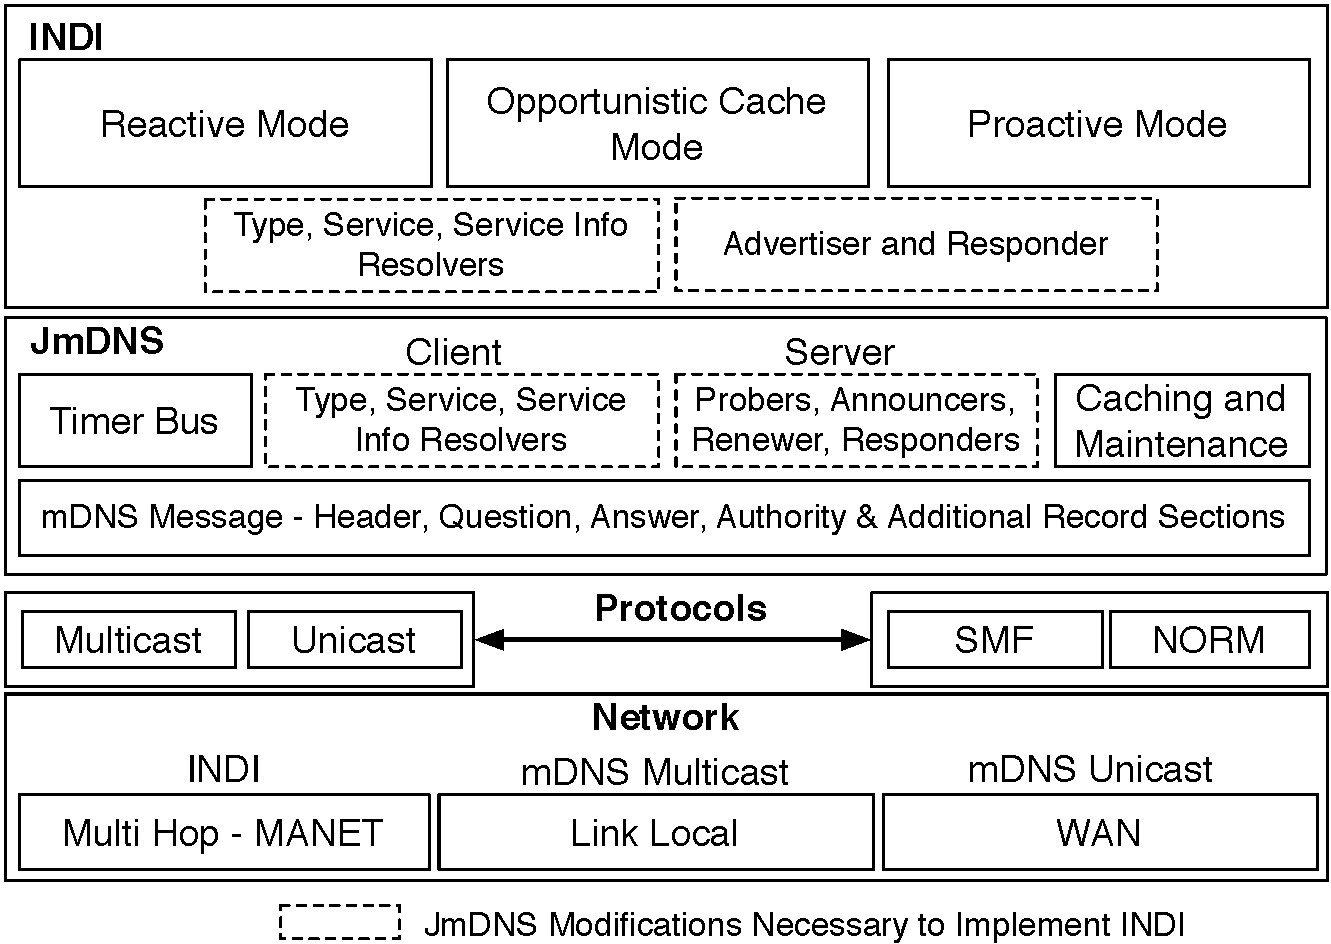
\includegraphics[scale=0.55]{INDIArchitecture.pdf}
%\vspace{-8pt}
\caption{INDI Architecture} \label{indi:fig:architecture}
%\vspace{-20pt}
\end{figure}

Figure  \ref{indi:fig:architecture} shows the resulting architecture for INDI taking into consideration the INDI design specification and the mDNS entities used to implement the mDNS functionality.  This architecture shows a schematic for the layering of the INDI design profiles: reactive; opportunistic cache; and proactive, onto the existing advertiser and responder, type, service, info resolvers.     It can be seen that for the client side, JmDNS entities are similar to INDI, the major differences being in the number of resolvers deployed and the timings of retries to support the INDI design configurations.  However, the server side protocol is significantly different with INDI only requiring advertising and responding roles compared with JmDNS that has probe, announce, responder and renew roles.  The advertising role in INDI is a simplification of the probe, announce and renew roles in mDNS.

The rest of the software architecture mimics JmDNS as illustrated in Figure  \ref{indi:fig:architecture}. Once packaged by the different entities, the message format can use the same messaging serializer and on-the-wire format to remain compatible with DNS.  INDI therefore should be 100\% JmDNS/mDNS, AVAHI and Bonjour interoperable.   

For the networking level, the conventional deployment of JmDNS and INDI differs considerably. Whilst on a static infrastructure LAN, the protocols being used would be standard multicast and unicast, on a MANET, these underlying protocols would generally be replaced by more flexible and adaptive protocols to cope with the changing infrastructure more effectively. An issue that impacts critically here, is the link-local scoping of  mDNS that forms part of the specification.   Therefore, since mDNS is intended for link local operation and there are presently no de facto standards or accepted addressing practices for extensions to site-local or multi-hop ad hoc network operation, we also support ``proof-of-concept'' multi-hop operation through a SMF (Simple Multicast Forwarding) \cite{macker2004simplified} plugin, which forwards mDNS messages for site-scoped  areas, where mobile ad hoc routing may require highly dynamic edge routing.  This solution provides an administratively scoped multi-hop capability versus the more typical single network hop IP link-local multicast capability used by many deployed service discovery approaches.  

These same types of optimized flooding algorithms are also available in many ad hoc routing control planes and existing research has demonstrated the ability to encapsulate service discovery messaging within the control plane mechanism \cite{li-lightweight}. We do not suggest a particular approach to the message forwarding here, as there are many valid options and INDI supports standard IP multicast traffic that can also be adapted for middleware encapsulation.  Rather, we focus on examining the use of such techniques, whether encapsulated or not, to enable the potential for more robust distributed querying, response, and proactive notification.

%For example, previously we have used the Essential Connected Dominating Set (ECDS) algorithm \cite{Macker:2007:SMFCDS} in deployment for multicast routing.  Here, the backbone is calculated in a distributed manner based on localized neighbor information and the selected CDS algorithm.  Selected nodes rebroadcast all non-duplicate multicast packets providing network wide flooding for all multicast traffic.  

\subsection{Implementation}
\label{sec:implementation}

We have been working closely with the JmDNS community \cite{jmdns} provide a pluggable architecture in JmDNS for INDI to be able to provide different functionality for the mDNS entities described in Section \ref{sec:requirements} for overlaying INDI profiles (see Section \ref{sec:architecture-design}).  The JmDNS \cite{jmdns} authors provided customization of the Java timing interfaces to the JmDNS entities for our use to integrate custom tasks for layering INDI modes, which is shown in Figure  \ref{indi:fig:architecture}.   
    
For the entities, we replace the \emph{Prober}, \emph{Announcer} and \emph{Renew} tasks with an Advertiser class, which performs the proactive advertisements as and when they are required.  A and AAAA records are not included in the advertisements because in a MANET, other address mechanisms are in place to avoid potential conflicts here.  INDI includes a modified \emph{Responder} for replying to tasks, which switches between unicast and multicast depending on the mode we are working within i.e. for Opportunistic cache and Proactive modes the responder replies with a multicast message and in Reactive, it replies with a unicast message.

On the client side, the type, service and service info resolvers resemble the JmDNS variants with three main differences.   INDI resolvers always check the cache before sending out queries to the network.   Secondly, the sequence of solicitations for resolving queries is different.  A user can specify any sequence they choose in INDI so this is a user preference depending on the application.  Third, the responses from the resolver are far more aggressively propagated to the resolvers in INDI.  This results in less queries being sent because as soon as a reply to a query has been received, the resolver quits operation.     
 
There are other housekeeping classes that differ in the INDI implementation.    We have the INDI \emph{Canceller} that can be customized to send out packets onto the network at whatever interval a user chooses or can be turned off to act in a completely passive manner and allow the TTL to expire the advertisement.  For example, for the experiments in Section \ref{sec:methodology}, we do not send any cancel messages onto the network because the TTL is so short we do not need further proactive behavior from the other components.  Instead, we use the INDI \emph{RecordReaper}, which is far more aggressive than the JmDNS counterpart.  Reaper intervals can be specified in the configuration depending on the frequency one would like to check the cache and expunge out of date advertisements.  For JmDNS, this is generally performed to coincide with other requests but in INDI one can program it to check at the millisecond level.   For the experiment described in  Section \ref{sec:methodology}, we use a reaper interval of 500 milliseconds. 

INDI provides a profile structure that build up layers according to the profiles defined through combinations of the core parameters defined in the previous section.  The Java class \emph{Profile} provides rudimentary defaults for all modes.   Client query intervals (for the resolver implementations) are set to trigger at 0, 100, 200, 400, 800 and 1600 milliseconds, respectively. The default TTL is set to the the mDNS specification recommended value of 2 hours and the readvertisement interval is set to half that value, also as recommended in the specification.  These defaults are inherited  by the \emph{Reactive} class, which exhibits the most similar behavior to mDNS.   The \emph{Opportunistic Cache}  profile also inherits the same behavior as \emph{Reactive} but it differs in that it responds to queries using multicast so that other INDI nodes can opportunistically cache the results. It also differs in that it does not proactively request a service until it first checks its cache to see if one that matches has already been cached (by using the Send Wait Interval).

The \emph{Proactive} profile, on the other hand, is significantly different.  First, the TTL value is generally a lot shorter.   For the experiments, we describe in Section \ref{sec:methodology}, we use a TTL of 2 seconds and a readvertisement interval of 1 second.   Second, the endpoints are always included in the proactive announcements because the readvertisement rate is so high that the endpoints are constantly refreshed anyway. Therefore the resolvers generally are never need to send out resolver queries, so the sequence of resolver timeouts is changed to make sure the cache is checked before any resolving sequence takes place.  
  


\section{Experiment Background and Emulation Environment}
\label{sec:core}
In the experiments discussed in this \doctype, we expand on previous experiments, described in Section \ref{sec:indi}, by applying JmDNS and INDI to a full emulated scenario that is designed to empirically measure the differences in message overhead and latency for a realistic scenario.  Therefore, for the experimental evaluation in comparing the performance of INDI and JmDNS, described in \ref{sec:methodology} and \ref{sec:results}, we used the CORE Emulation framework \cite{ahrenholz2008core}. 

The Common Open Research Emulator (CORE)  is a network emulator that runs real computer networks in real time.  This is quite distinct from  simulation (e.g. ns-2 \cite{NS2_webpage}), which builds a model of a real network and then triggers events at discrete time intervals in order to simulate a actual application's use of that network.    Although simulators can be used to provide targeted empirical evaluations, generally most experiments are limited in scope and provide very focused and controlled experiments which make a number of functional assumptions compared to what a real application might do.   Therefore, the deployment of such applications in real-world environments can often be problematic and lead to a number of unmeasured issues and bugs that are caused by both the application's software implementation (code issues, multi-threading, socket performance, etc) and underlying network problems that can significantly affect performance.  Consequently, and timely due to the growth and maturity of lightweight virtual machine implementations, we have chosen to use the CORE emulation environment for our INDI experiments, in order to to gather real-world deployment experience for moving to production quality more expeditiously. 

Briefly, CORE has two components:  a CORE services (daemon), which manages the emulation sessions and interfaces with the underlying Kernal virtualization; and the graphical user interface, which is a drag and drop GUI that can be used to orchestrate the creation of the nodes. These two components communicate using an asynchronous, sockets-based CORE API, which is written in Python. 

The Core services daemon, on Ubuntu 11.04, interfaces with Linux network namespaces virtualization to build its virtual nodes. Linux namespaces builds up from chroot to implement complete virtual systems, adding resource management and isolation mechanisms to the existing process management infrastructure.  The result is that each node is a lightweight virtual system with full resource isolation and resource control for an application; that is, each node essentially provides a lightweight virtual machine, which can all access a common host filesystem (although permissions can be set so that some directories are private on a per-container basis).  Linux network namespaces (netns) is part of the mainline 2.6.27$+$ Linux kernel.
 
From a network perspective,  each namespace has its own loopback device and process space. Virtual or real devices can be added to each network namespace, and you can assign IP addresses to these devices and use them as a network node.  The virtual networks are built using the Linux Ethernet bridging and for the Wireless implementation we use here, employ the use of OSPF routing protocol configurations  using the Quagga \cite{quagga} open source routing suite.  The MDR router type in CORE builds OSPF MANET Designated Routers (MDR) configurations which requires a modified version of Quagga \cite{ospf-mdr}.   Quagga OSPFv3 is such an implementation of  OSPF MDR \cite{rfc5614},  OSPF Database Exchange Optimization \cite{rfc5243}, and  OSPFv3 Address Families \cite{rfc5838}, for efficient routing in mobile ad hoc networks (MANETs).



\section{Service Visualization}
\label{sec:protosd}
The INDI discovery systems is currently being used for chat and multimedia applications in the Naval Research Lab \cite{Macker2010a, Dean2011}.  It provides low level modes for service discovery in mobile networked environments and provides interfaces for allowing applications to use this functionality to enable end-to-end connectivity.  In this section, we describe ProtoSD, which is the operating and service visualization environment for INDI and outline some of the applications that are INDI is motivated by. 

Proto Service Discovery (ProtoSD) is a toolkit that provides a single homogeneous toolkit for running both the mDNS and INDI discovery systems.   ProtoSD has a: command-line interface modeled using Apple's ``mdns'' command line tool for Bonjour; file-based interface for allowing third party applications to be integrated; and a Web-based interface for dynamic visual representation of the discovered services through a conventional Web browser.   The file interface and Web interface are the two most commonly used.  For the file interface, ProtoSD can optionally be used to generate ``.services'' files,  providing a simple file-based API for other applications to interface with e.g. we are currently using this with Python to read the ``.services'' file and provide a TV channel for incoming videos.  It also allows a single sink application to read services from multiple sources on a shared file system, which enables service browsing in CORE .  Our two main usages therefore are:

\begin{description}
\item [Private Service Browser:] by running the ProtoSD Web component locally and  browsing the network using the command line with a ``-g'' flag, ProtoSD enables the back-end Web server to provide a dynamic updated view of the services.  
\item [CORE Service Browser:] using CORE's shared file system, it is possible to use ProtoSD to show the services being discovered on all CORE nodes simultaneously using one browser.
\end{description}

For private browsing, ProtoSD passes service discovery and removal announcements directly to the command line or Web browser component for visualization, whilst for CORE, the ProtoSD file interface is used to bridge between CORE and the host Web browser.    Each CORE node stores its discovered services  in ``/tmp'' within ``.services'' files (named after their node name and network interface). The host scans this directory for write updates and loads all files simultaneously for rendering in a Web browser. Since the CORE nodes are not easily connected to the host, this simple shared file based mechanism provides a convenient way of visualizing the services without needing to reconfigure the default set up of CORE.   Using this approach, one can give a global view the services dynamically as and when services are advertised and removed from the network.  All of the emulations described in Section \ref{sec:results} used ProtoSD to visualize the output as the emulations were taking place.  This also provides a quick-look verification mechanism for ensuring the runs were operating normally and thus expedited the process.   

\begin{figure}[h!]
\centering
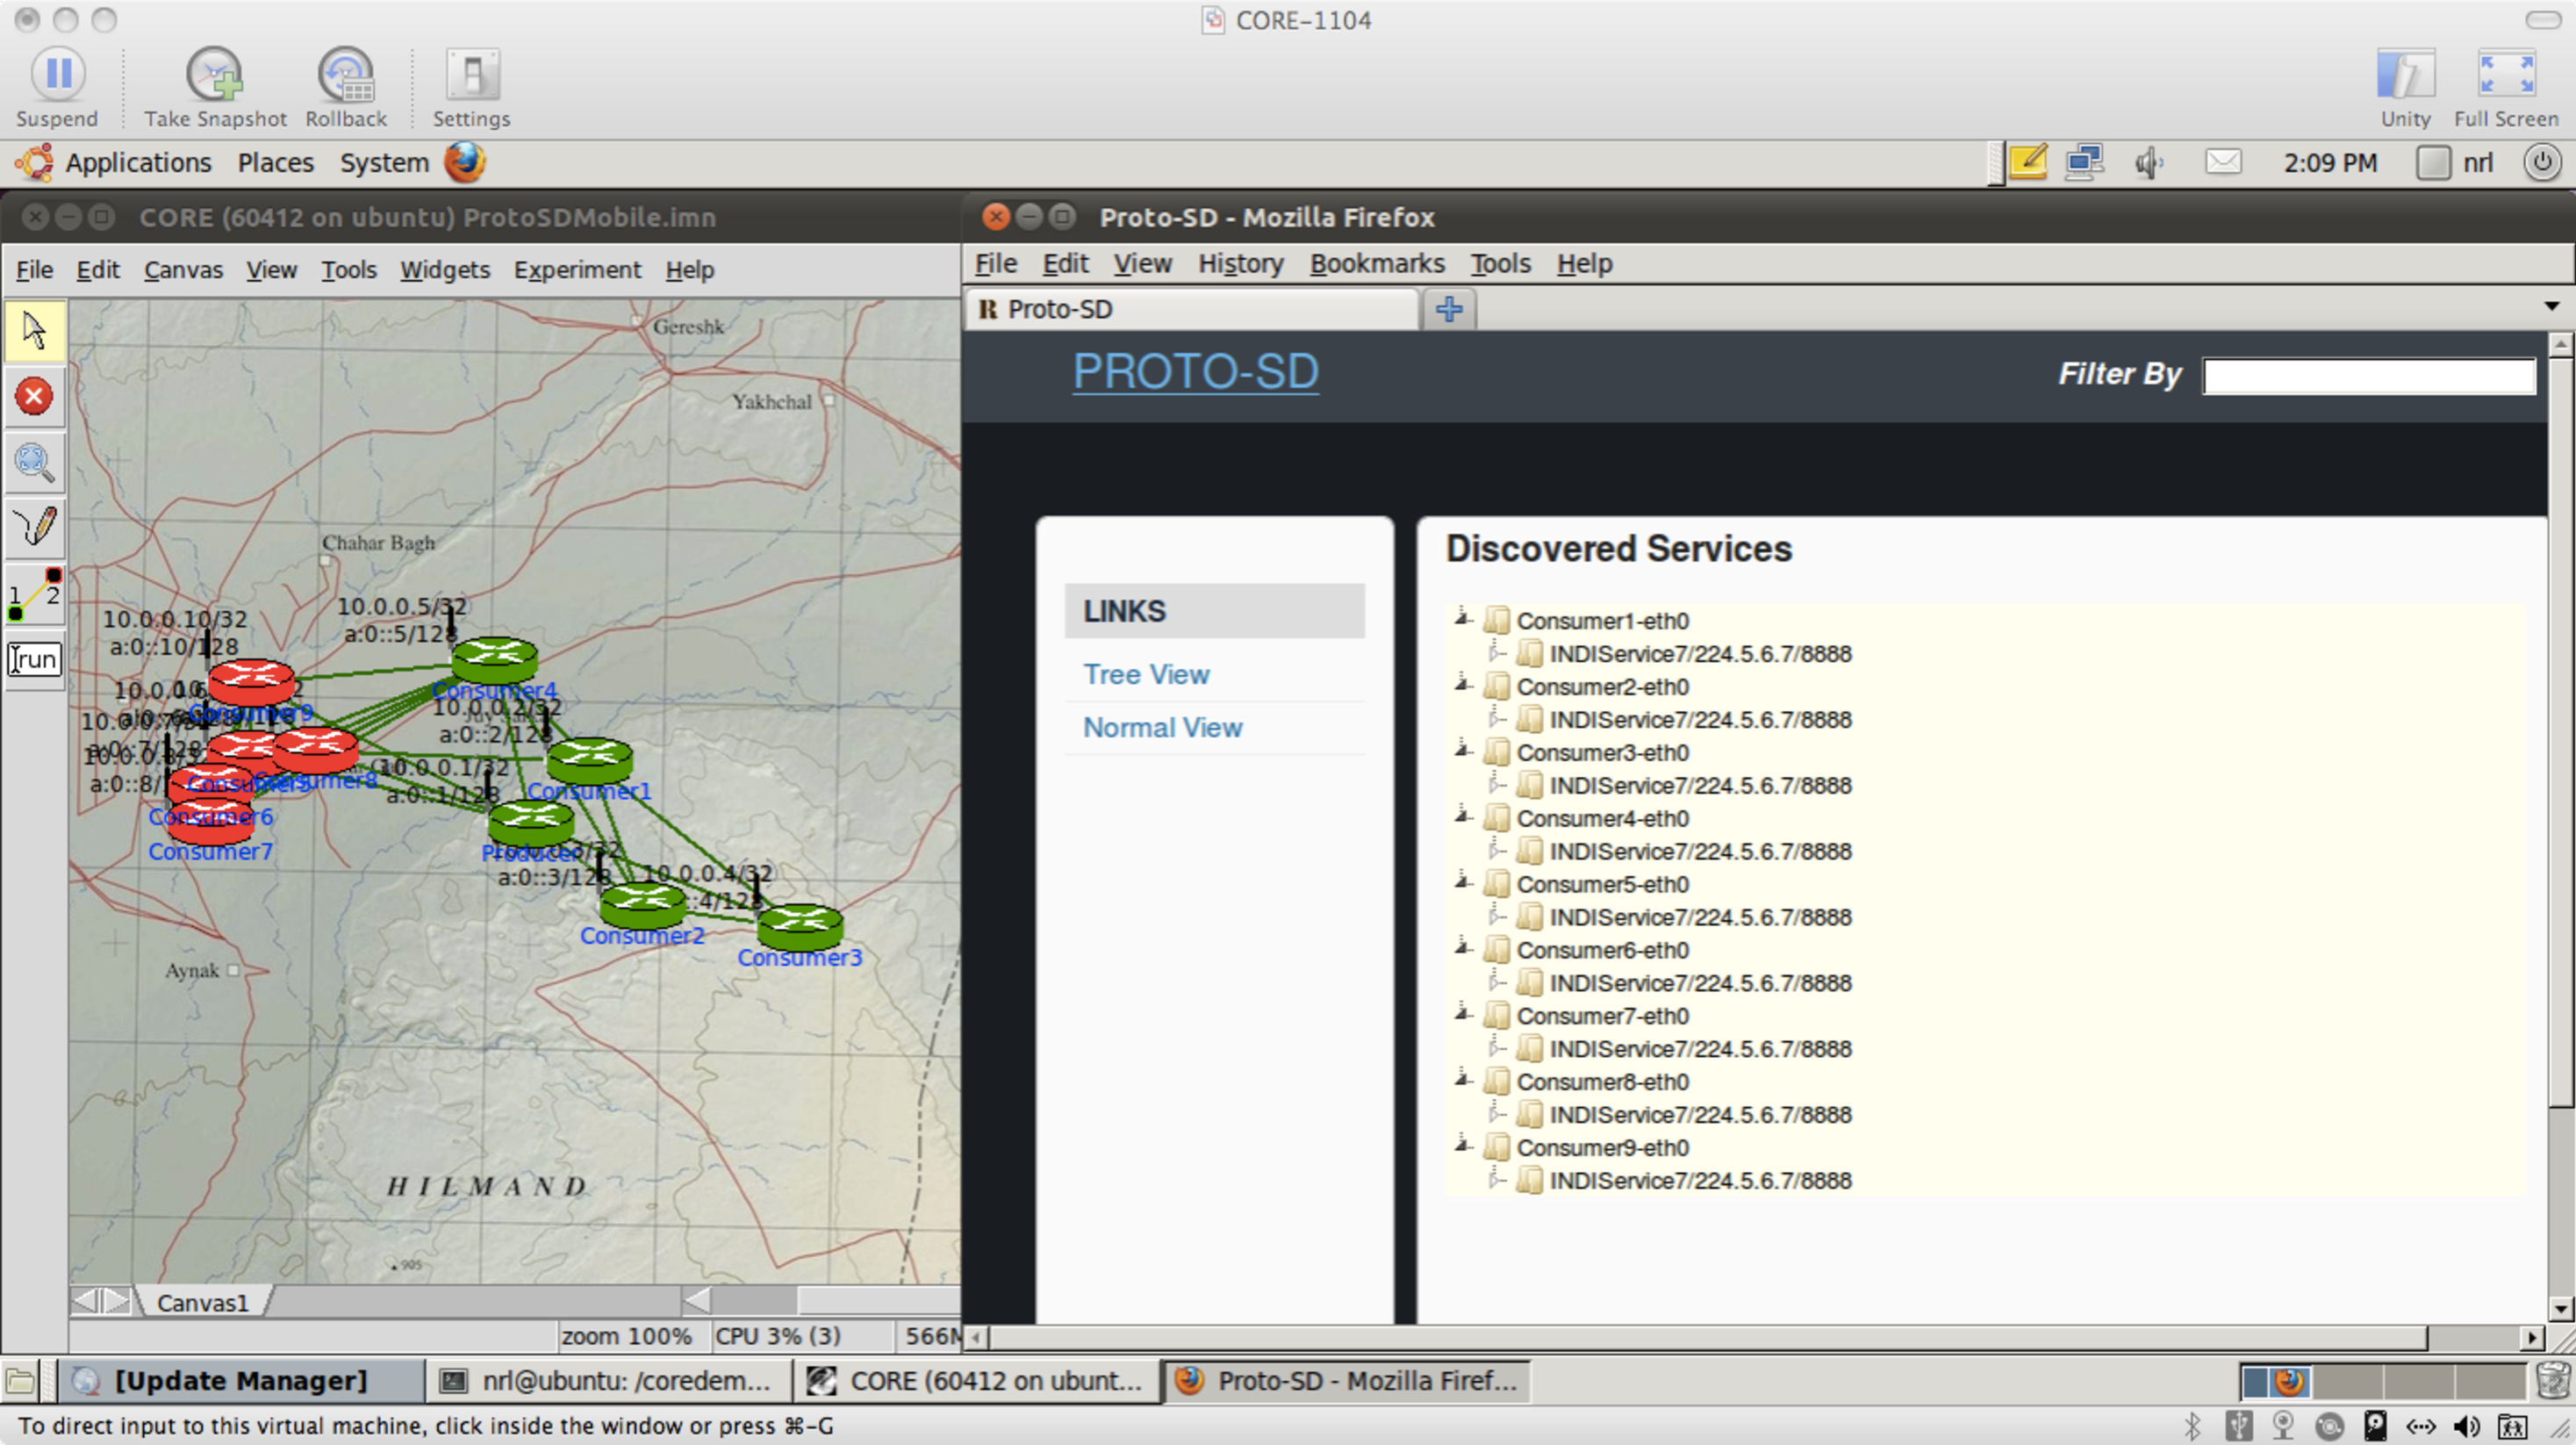
\includegraphics[width=5.5in]{ProtoSDCore.pdf}
\caption{ProtoSD running in CORE showing the services discovered during one mobile emulation for the INDI discovery system.} 
\label{indi:protosdcore}
\end{figure}

On the right hand side of Figure \ref{indi:protosdcore}, we show a screenshot of the ProtoSD Web interface, displaying the services it has discovered from each consumer in a CORE emulation in a tree view.  ProtoSD uses a Java-based lightweight Web server framework, called Restless\footnote{Restless was developed by Andrew Harrison, now working for  the Carefx Corporation but not yet released publicly}, for exposing the backend services.   Restless is a simple HTTP 1.0 compliant Web server that is capable of delivery multiple types of data efficiently and providers virtual endpoints for representing services using REST facilitating the Create, Read, Update and Delete (CRUD) style of operations.  To enable dynamic updates, ProtoSD uses a client-side JQuery component \footnote{http://jquery.com/}  that queries the server using an AJAX asynchronous HTTP GET to return service advertisement updates as and when new services are available. In this way, the browser updates immediately upon discovery of a new service (i.e. uses the COMET style\footnote{http://en.wikipedia.org/wiki/Comet\_(programming)} of server callback). By exposing two independent endpoints for fetching a JSON or HTML data structure from the server, it can render  using either a JsTree\footnote{http://www.jstree.com/} JQuery tree structure or HTML, for displaying to the users. Using the ``search'' textfield at the top right allows pruning of this list to match only the provided string.  

\begin{figure}[h!]
\centering
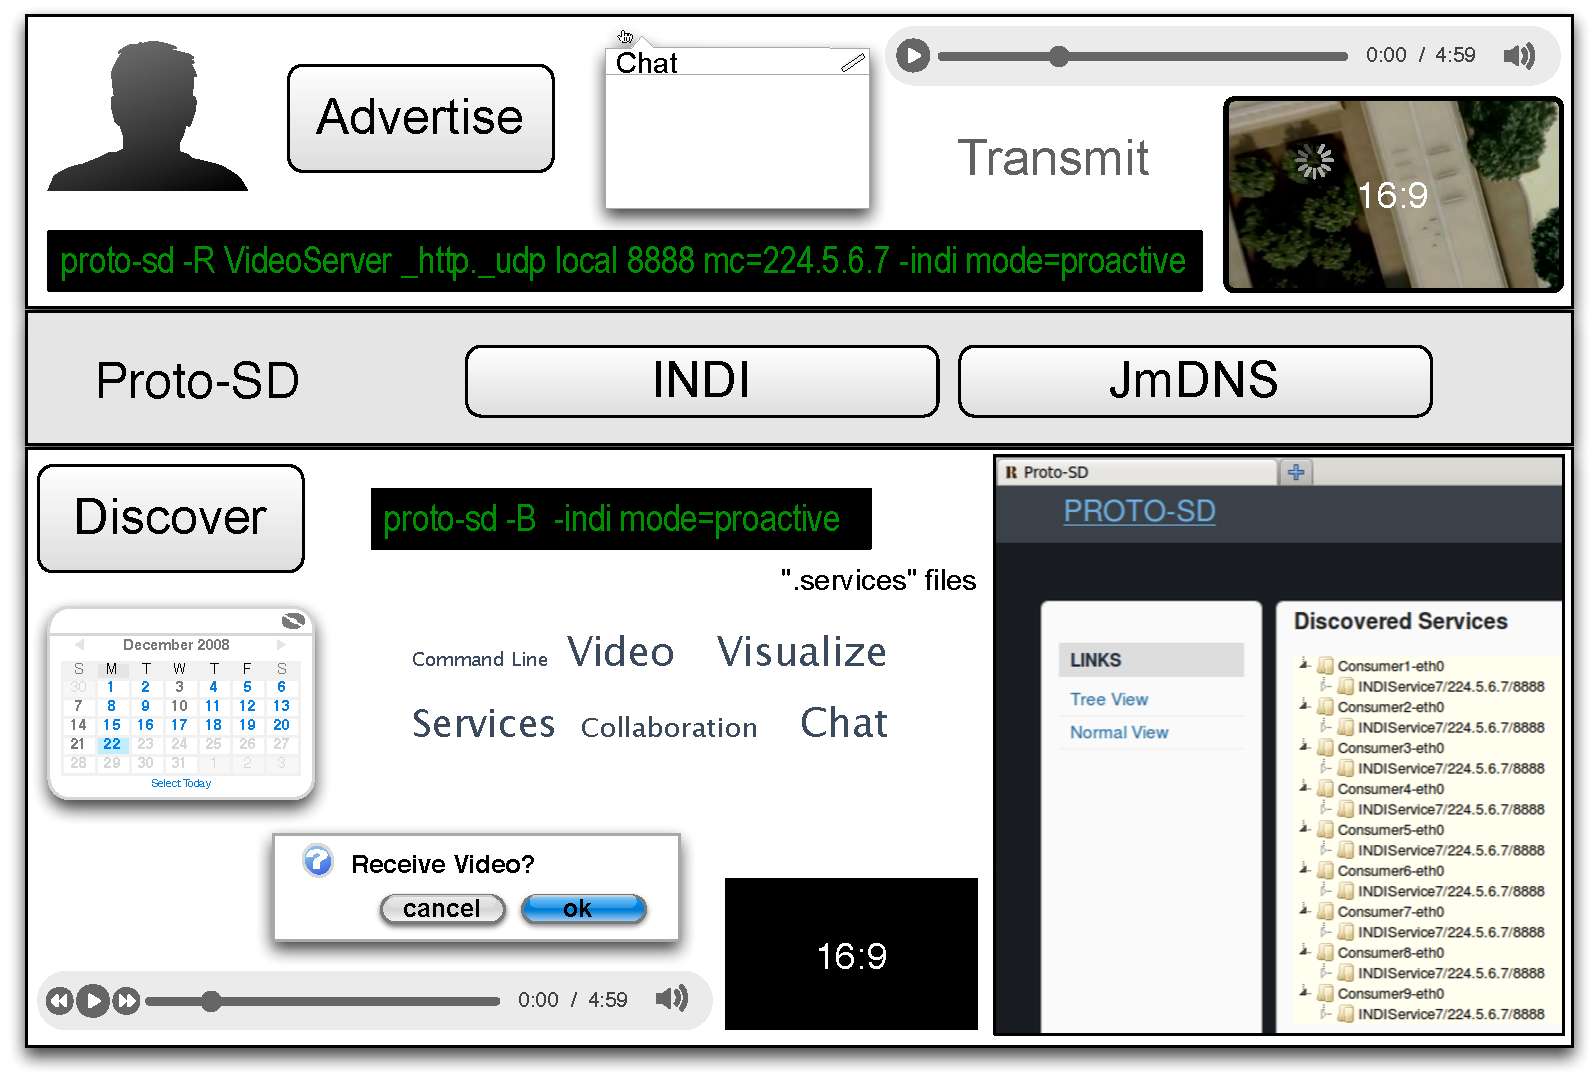
\includegraphics[width=5.5in]{ProtoSD.pdf}
\caption{An overview of ProtoSD showing the interfaces by which services are advertised and how services can be discovered and visualized.   We also show the kinds of applications ProtoSD has already been implemented with.} 
\label{indi:protosd}
\end{figure}

Figure \ref{indi:protosd} shows an overview of the various components involved in advertising and discovering using ProtoSD and some of the application use cases.   ProtoSD has been used as a private browser for discovering multimedia (video and audio) streams and providing an interface for allowing clients to connect to them using video toolkits (e.g. VLC\footnote{http://www.videolan.org/vlc/}).  For some applications, the Web GUI also provides an off-the-shelf solution for exposing management information about the participants in the network.  For example, for an XMPP multi-user chat (MUC) session, the ProtoSD browser can be used to provide a similar mechanism to what centralized XMPP management servers provide for administrators. Using OpenFire\footnote{http://www.igniterealtime.org/projects/openfire/}, an administrator can view the current MUC rooms created by users that are currently connected to this server.   For ProtoSD, the MUC rooms that are created by its users also appear as adverts on the multicast network and are consequently discovered by ProtoSD and listed through the Web GUI accordingly.  ProtoSD and INDI have already been used for this purpose by integrating with the XOP\cite{xop2010} serverless XMPP chat system on a MANET. 



\section{Experiment Methodology}
\label{sec:methodology}

All experiments performed in this \doctype~were running CORE, described in Section \ref{sec:core}, on an Ubuntu 11.04 virtual machine hosted using VMware Fusion on a Mac Air laptop. The experiment emulates a 10 node wireless networking mobile scenario, which consists of 9 consumers (nodes that want to discover a particular service) and 1 producer (a node that wants to advertise a service for use by others).   The mobility patterns for this scenario were generated using an ns-2 mobility pattern generator and then imported into CORE using its inbuilt ns-2 mobile script importer. The emulation runs for 250 seconds and for mobility purposes, the nodes where split into two distinct groups with 5 nodes per group: the first group containing consumers 1-4 and the producer; and the second containing consumers 5-9 inclusively. A screenshot from the CORE GUI representation of this scenario is provide in Figure \ref{indi:fig:core}. The mobile network has a range of 200 meters and a bandwidth of 54 MHz and the entire surface for the emulation covered a surface of  330,000 square meters (600 x 550) with a maximum speed of each node being 20 meters per second. The two clusters of 5 nodes fragment and coalesce around every 30 seconds and therefore there are 4 fragmentations, where the two groups go out of range from each other, during the entirety of the emulation.  This is discussed further in the next section.

\begin{figure}[h!]
\centering
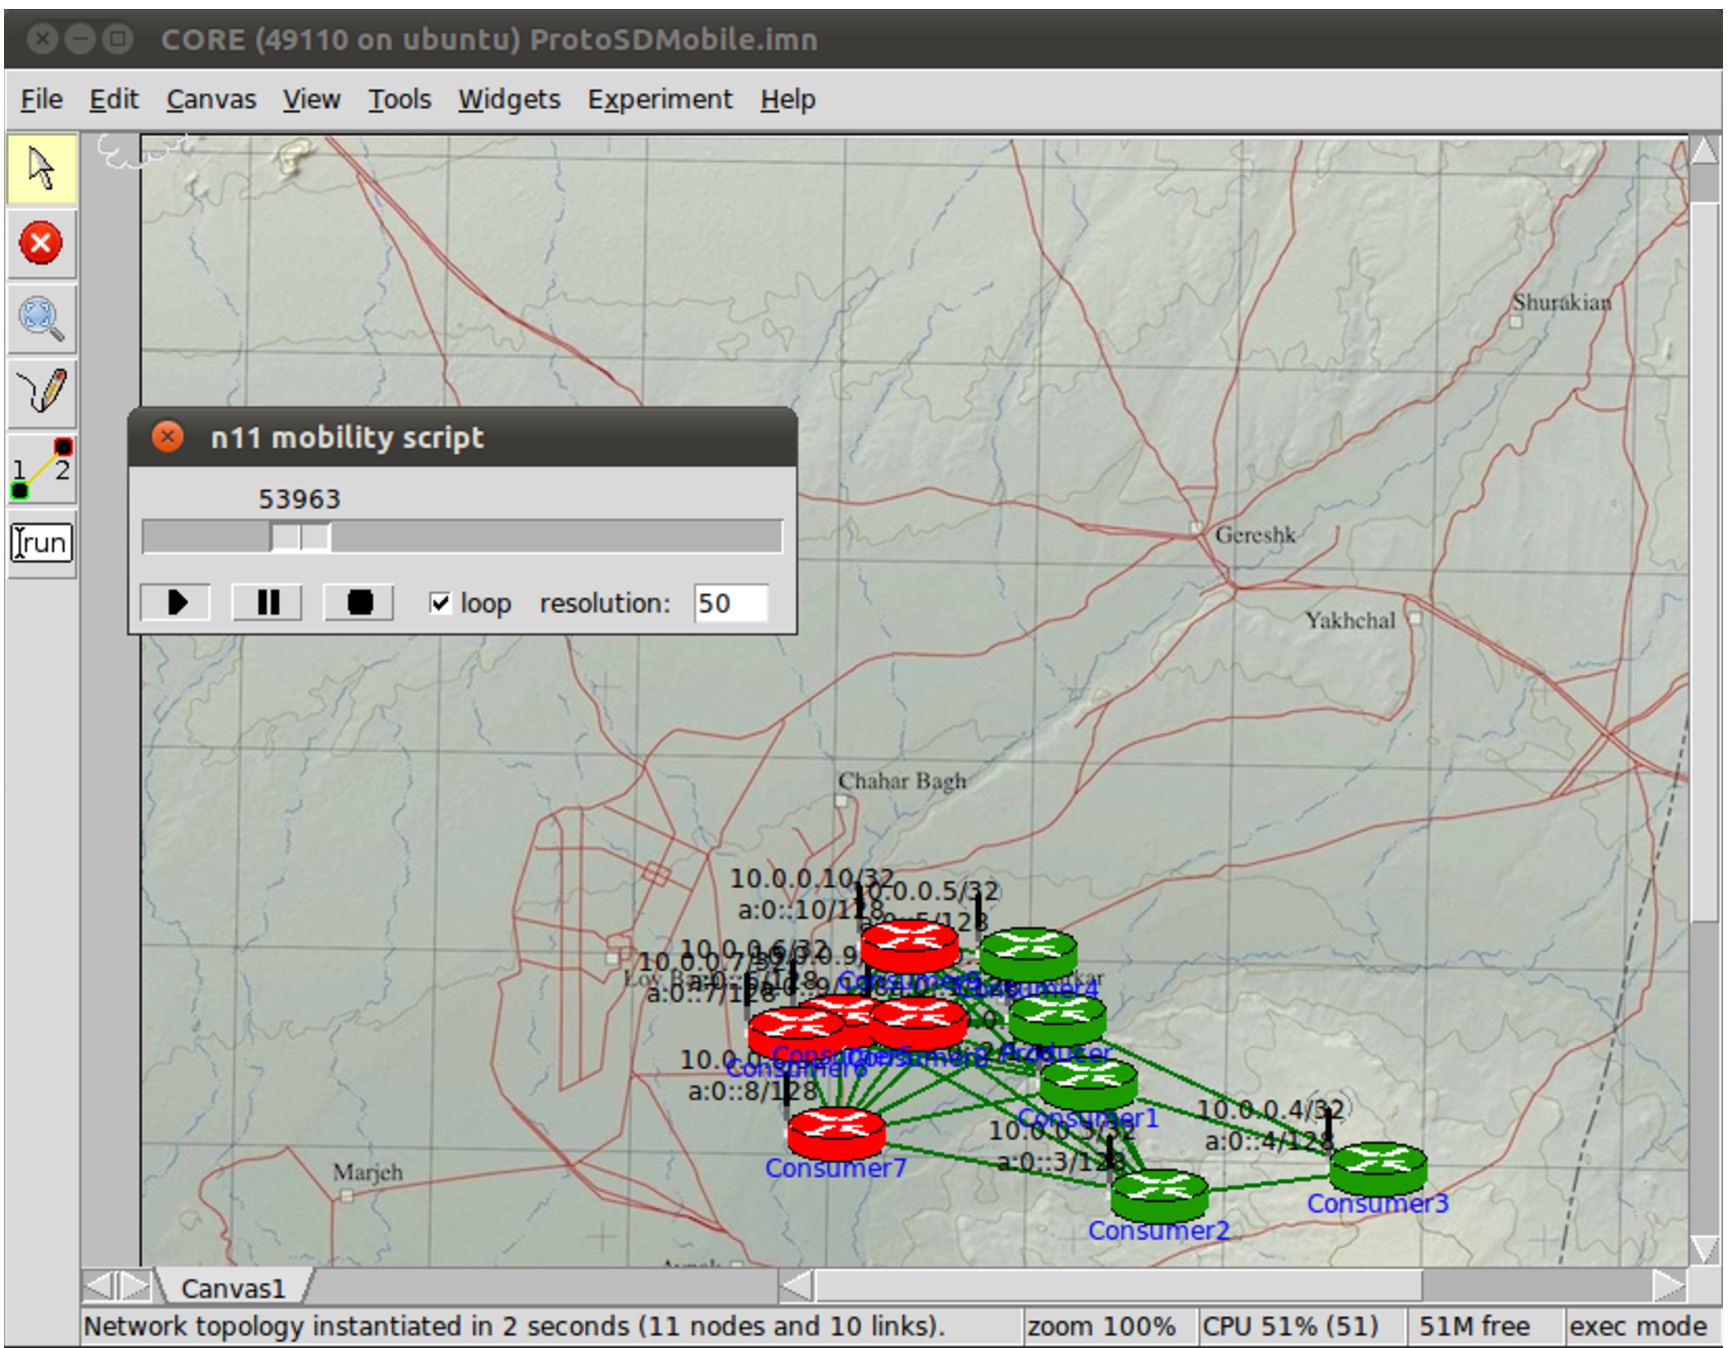
\includegraphics[scale=0.45]{COREEmulation.pdf}
\caption{The running CORE Emulation showing 9 clients and one service running INDI} 
\label{indi:fig:core}
\end{figure}


\subsection{Data Collection}

To collect data from the live emulation experiments, we implemented a distributed file-based event mechanism that gathers information about the low-level packets alongside the higher-level discovery events for each CORE node in a consistent fashion and common format.  Data is collected using one line per event and stored as Comma Separated Values (CSV) for quick-look analysis in Excel and convenient post processing using Java and bash scripts. The CSV files from all CORE nodes are collected in ``tmp/protosd-current'' and time is synchronized across all nodes, which is triggered by the pressing of ``Play''  for initialing the mobility pattern in CORE. This ensures the timing consistency between multiple runs. We record three levels of events:

\begin{description}
\item [At the Packet Level: ] Packet level events are measured using a Java ``tcpdump'' unix process on every core node that records all packets transmitted on the mDNS multicast address (224.0.0.251) on ``eth0'', which is the wireless interface on each CORE node on the emulation.    Packet events store the core node the packet was measured on, the message identifier and its length (in bytes).   The packet level events are used to record the traffic across the course of the emulation in order to construct traffic histograms showing the traffic  at each time-step of the experiment. 

\item [At the Discovery Level: ] Discovery level events record the arrival and departure of services during the course of the emulation.  Service events are recorded from a service producer (when an advert is advertised and removed) and from a consumer (when an advert is resolved and removed)

\item [Multicast Pings: ] In order to automatically detect the mobility pattern during the course of the emulation, we first observe (as a separate run) multicast ping events.  The ``multicast ping'' does not follow the ping protocol but offers a similar level of functionality by sending out packets that can be used to detect whether a server is reachable or not at any given point of time.  In the case of multicast and the one-to-many relationship, we send a multicast message from the producer node to the mDNS multicast address.  All consumers join this multicast group and listen for responses.  
\end{description}


\begin{figure}
\centering
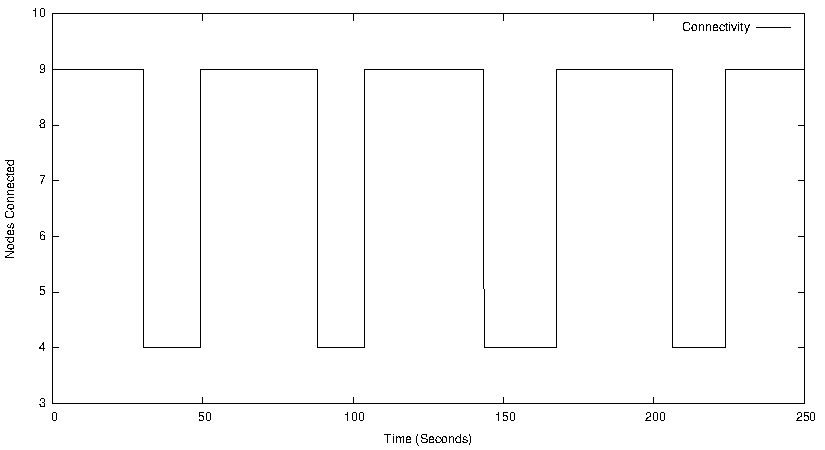
\includegraphics[scale=1.0]{indi10ping-distribution.pdf}
\caption{The connectivity of the two groups of nodes during the course of the 250 second emulation.  The nodes fluctuate between 9
consumers and 4 consumers when the two groups split.} 
\label{indi:fig:emulationconnectivity}
\end{figure}

Multicast ping messages are sent out 10 times per second and we record the event as and when they are received by each consumer to record when each consumer is reachable from the producer.  Ping packets contain an identifier (a simple incremental counter from the producer) along with the sender name. The multicast ping events provide us with a 100 millisecond connectivity matrix for the entire duration of the emulation, which is extremely important, as it allows us to calculate a theoretical limit for the optimal success rates that should be achievable by the service discovery systems.  The result of the ping events can be seen in detail in Figure \ref{indi:fig:emulationconnectivity} for the mobility pattern we used in the emulations.  Multicast ping events are used to generate a histogram that shows the number of consumers that are ``connected''\footnote{The term connected here simply means that a consumer node should be able to receive multicast packets from the producer - it does not imply any protocol-specific usages of this term e.g. TCP.} to the producer at a particular point in time. Therefore, Figure \ref{indi:fig:emulationconnectivity} shows that the number of consumers that are within a multi-hop reachable path of the producer fluctuates between 9 and 4 nodes at the times shown by the X axis of this figure.   This reflects the two distinct groups and the points in the graph where only 4 nodes are connected represents a fragmentation of the two groups.  Therefore, there are 8 transitions during the emulation where the two groups of nodes fragment and then rejoin.   

\subsection{Service Advertisements and Qualitative and Quantitative Metrics}

To measure the responsiveness of the service discovery system for detecting the arrival and departure of services in the face of network fragmentation and dynamics, we generate a sequence of finite-length service advertisements during the course of the emulation.  The adverts are sequentially numbered in chronological order and are named  according to the discovery system that is being used for a particular test (e.g. INDI or mDNS).   For terminology, each advert ``arrives'' in the network when it is advertised and ``departs'' from the network when that service advertisement is removed.    Services are sequenced according to a Poisson distribution and split into three sets with a mean interval of 10, 20 and 30 seconds.  When one advert is advertised the previous advert is simultaneously removed.  

\begin{figure}
\centering
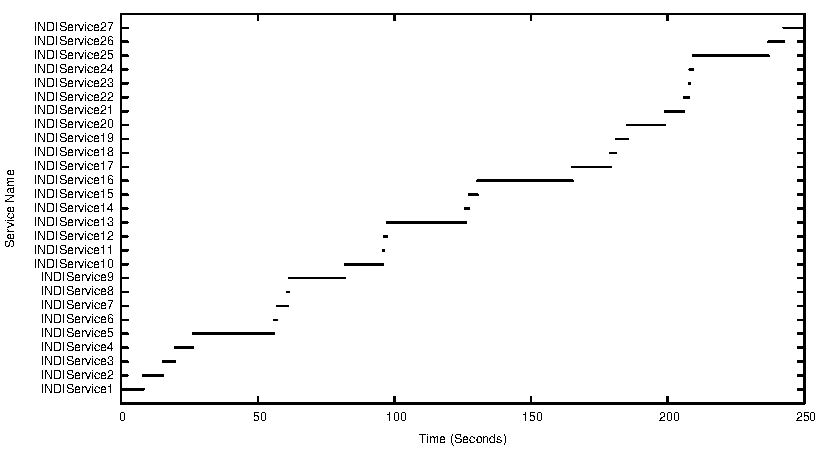
\includegraphics[scale=1.0]{indi10advert-distribution.pdf}
\caption{Shows the time and duration (x axis) that each of the named services (y axis) are advertised for during the emulation.} 
\label{indi:fig:poisson-10-adverts}
\end{figure}

A pictorial representation of the time and duration of services advertised in an emulation, with a Poisson mean interval of 10 seconds, is provided in Figure \ref{indi:fig:poisson-10-adverts}. This diagram shows the emulation time (in seconds) on the x-axis and the name of each service advertised, sequenced by service name and hence arrival time, on the y axis.  In this particular emulation therefore, there are 27 service advertisements during the 250 second emulation, which exhibit Poisson behavior with respect to the time duration they are advertise for.   

In a Poisson exponential probability distribution, the time interval from the current time to the occurrence of the next event does not depending upon the time of occurrence of the last event. This provides a somewhat realistic distribution for modeling real-world random events, such as the arrival of service advertisements in a number of application scenarios. For the same reason, Poisson is often used to model customer arrivals that trigger requests for stress testing web servers.

\begin{figure}
\centering
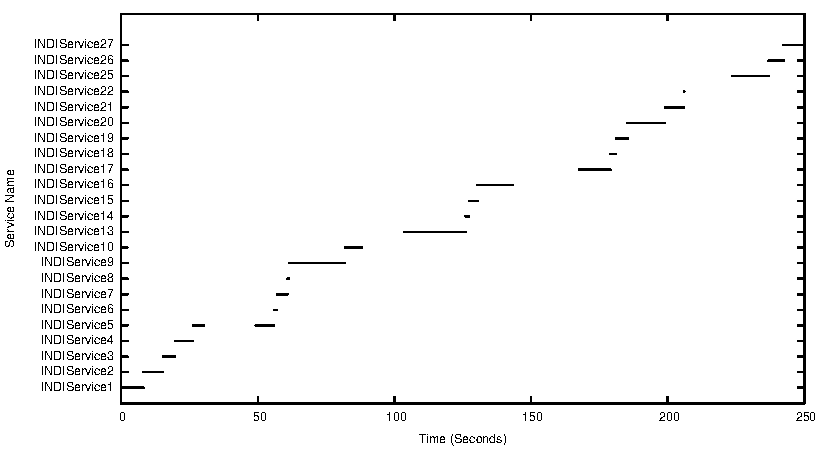
\includegraphics[scale=1.0]{indi10advert-distribution-fragmented.pdf}
\caption{Shows the time and duration (x axis) that each of the named services (y axis) are available for to the fragmented nodes during the emulation.} 
\label{indi:fig:poisson-10-adverts-frag}
\end{figure}


Figure \ref{indi:fig:poisson-10-adverts}  shows the service view from the producer side (server side), which although is also consistent with the permanently connected Consumers 1-4, does not show the consumer view for Consumers 5-9 -- the group of consumers that get fragmented according to the distribution shown in Figure \ref{indi:fig:emulationconnectivity}.  During times of fragmentation therefore, the possibility of discovering the advertisements becomes even more restricted and if we apply this connectivity matrix to the service distribution, we obtain Figure \ref{indi:fig:poisson-10-adverts-frag} that illustrates the actual availability of services advertisements for nodes 5-9 after the fragmentation has been applied to the network.  As one can see, during the periods of fragmentation several adverts e.g. INDIService11, INDIService12, INDIService23 and INDIService24, are not available to these consumers.   

For analysis, the ping traces that are applied to the Poisson distributed service advertisements provide a unique multidimensional view for each consumer with respect to the underlying network behavior and therefore we should take the following two key issues into account when defining the metrics for such an experiment:

\begin{itemize}
\item  \textbf{Optimal Performance:}  If the fragmentation perspective shown in Figure \ref{indi:fig:poisson-10-adverts-frag} is applied algorithmically when analyzing the data, we can calibrate the results according to the optimal discovery performance a service discovery system ``could'' achieve for each service distribution. Therefore, a score of 100\% should be achievable by a system that meets the design constraints of dynamics of the underlying network.  

\item \textbf{Accurate Service Detection:}   Since service distribution can be calibrated to the underlying network connectivity, we also have an accurate Consumer's view of the both the arrival and departure of services. Therefore, a success metric should take into account both the Service Discovery System's ability to detect the arrival of a service and the ability to detect when it is no longer available.
\end{itemize}

As one can plainly see therefore, simple metrics therefore, such as ``success rate'' for discovery and the ``latency'' taken for the service discovery system to discover a service are insufficient for this experiment. In defining a rigorous scientific process for the evaluation of the results, it is important therefore to provide a model that calibrates the results with the above constraints to accurately get a picture of how optimal the system is.  For example, consider the following scenario: service A is advertised at second 2 of the emulation for 48 seconds.  Consumer1 discovers service A but then gets disconnected at second 4 of the emulation and returns in network view of service A at the 45 second on the emulation.  Clearly, here a service discovery system that states the service is available for the entire 46 seconds cannot be deemed successful because for 41 seconds, the service will be unavailable for use.   

A service discovery system therefore needs to track the services as they come in and out of range to give the consumer the highest accuracy possible to avoid service connection errors. In this \doctype, we use the notion of a ``Quality of Service'' (QoS)\footnote{http://en.wikipedia.org/wiki/Quality\_of\_service} to  define the success metric and then we record the latency of both the detection of the arrival and departure of a service.  

QoS is generally used in the context of networking and communication technologies and its goal is to (contractually) mitigate and eliminate unwanted impairments that impact the quality of voice, data and multimedia communications. Therefore, by applying a QoS metric to our service discovery systems, we are forcing a contractual commitment adhering to a certain level of service performance, robustness and reliability. This is in contrast to service discovery systems that happen to delivered on a �best effort basis�  i.e. without QoS guarantees. Therefore, the resulting QoS would naturally lead to a high quality of experience (QoE\footnote{http://en.wikipedia.org/wiki/Quality\_of\_experience}) for a user that wishes to use a particular service. This approach leads to the use of the following two parameters that control the QoS:

\begin{description}
\item[1. Service Discovery Detection for Service Arrival $SDD_{a}$:]   is a constant used to specify the maximum allowable number of seconds for the detection of the arrival of a service to the network.   
\item[2. Service Discovery Detection for Service Departure $SDD_{d}$:]   is a constant  is used to specify the maximum allowable number of seconds for the detection of the departure of a service from the network.    
\end{description}

\noindent and then the \textbf{Success Rate ($SR$)}  is a boolean (true or false) variable that is true if a service is discovered within the defined QoS,  specified below:


\begin{equation}\label{qos}
QoS \equiv (L_a < SDD_a) \wedge (L_d<SDD_d) 
\end {equation} 

where:

\begin{equation}\label{discovery-latency}
L_a= \abs{(D_a - A_a)} 
\end {equation} 

\begin{equation}\label{leaving-latency}
L_d= \abs{(D_d - A_d)} 
\end {equation} 

\noindent and

\begin{itemize}
\item \textbf{$A_a$} is the time the advert was advertised. 
\item \textbf{$A_d$} is the time of the departure of the advert. 
\item \textbf{$D_a$} is the time the discovery system discovered the advert. 
\item \textbf{$D_d$} is the time the discovery system discovered the departure of the advert. 
\end{itemize}

This QoS metric is applied to each of the 9 consumers after the connectivity matrix has been applied, in order to obtain an accurate percentage for the ``optimal performance'' a service discovery system should be capable of achieving for a particular set of services during the emulation. We believe this represents an accurate test for each system.

\normalsize

\section{Experimental Results}
\label{sec:results}

For the INDI and JmDNS comparison, we performed the following emulations and post processing analysis scenarios according to different QoS requirements:

\begin{description}
\item [Six Emulations:] consisting of three different emulations for each discovery system. Each emulation uses a different mean Poisson interval of 10, 20 and 30 seconds for generating the  events, which results in different advertisement periodicities and advert density rates during the emulation, i.e. 27, 15 and 7 advertisements are generated, respectively. The different emulations types are labelled Poisson-10, Poisson-20 and Poisson-30 and specific runs are labelled INDI-10, INDI-20, INDI-30, JmDNS-10, JmDNS-20 and JmDNS-30 for convenience.
\item [Ninety Six Analysis Scenarios:] which cover broad parametric range across the $SDD_{a}$ and $SDD_{b}$ parameters for specifying different QoS requirements. $SDD_{a}$ limits of 1, 2, 5 and 10 seconds and $SDD_{b}$ limits of 2, 5, 10 and 20 seconds were chosen (i.e. the total is 16 combinations for each of the 6 emulations = 96 cases).
\end{description}

\footnotesize
\begin{table}[h!]
\begin{center}
%\vspace{-5pt}
\begin{tabular}{| c | c | c | c | c | c | c | c | c | c |}
%p{1.1cm}
\hline
SDS-Interval & $SDD_{a}$ & $SDD_{d}(2)$ & $SDD_{d}(5)$ & $SDD_{d}(10)$ & $SDD_{d}(20)$  \\
\hline
INDI-10 & 1 & 82.89 & 93.42  & 93.42 & 93.42 \\
INDI-10 & 2 & 87.28 & 100  & 100 & 100 \\
INDI-10 & 5 & 87.28 & 100  & 100 & 100 \\
INDI-10 & 10 & 87.28 & 100  & 100 & 100 \\
\hline

INDI-20 & 1 & 68.0 & 96.0  & 96.0 & 96.0 \\
INDI-20 & 2 & 72.0 & 100  & 100 & 100 \\
INDI-20 & 5 & 72.0 & 100  & 100 & 100 \\
INDI-20 & 10 & 72.0 & 100  & 100 & 100 \\
\hline

INDI-30 & 1 & 70.51 & 87.18  & 87.18 & 87.18 \\
INDI-30 & 2 & 83.33 & 100  & 100 & 100 \\
INDI-30 & 5 & 83.33 & 100  & 100 & 100 \\
INDI-30 & 10 & 83.33 & 100  & 100 & 100 \\
\hline
\hline

JmDNS-10 & 1 & 0.0 & 2.19 & 2.19 & 2.19 \\
JmDNS-10 & 2 & 3.95 & 38.6  & 69.74 & 75.44 \\
JmDNS-10 & 5 & 3.95 & 38.6  & 75.0 & 80.71 \\
JmDNS-10 & 10 & 3.95 & 39.91 & 78.95 & 84.65 \\
\hline

JmDNS-20 & 1 & 0 & 0 & 0 & 4.00 \\
JmDNS-20 & 2 & 3.2 & 26.4  & 43.2 & 57.6 \\
JmDNS-20 & 5 & 3.2 & 33.6  & 50.4 & 64.8 \\
JmDNS-20 & 10 & 3.2 & 33.6 & 57.6 & 72.0 \\
\hline

JmDNS-30 & 1 & 0 & 0 & 0 & 0 \\
JmDNS-30 & 2 & 5.13 & 19.23  & 38.46 & 55.13 \\
JmDNS-30 & 5 & 5.13 & 19.23  & 38.46 & 55.13 \\
JmDNS-30 & 10 & 5.13 & 19.23  & 38.46 & 55.13 \\
\hline
\end{tabular}
\end{center}
\label{table:jmdns:comparison}
%\vspace{-15pt}
\caption{JmDNS and INDI Overview of Results.}
\end{table}
\normalsize

\begin{figure}
\centering
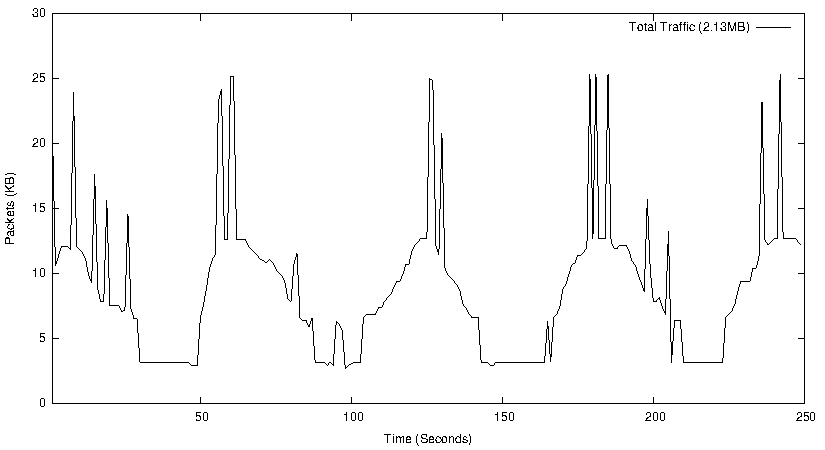
\includegraphics[scale=1.0]{indi10packet-distribution.pdf}
\caption{A histogram plotting the amount of network traffic INDI propagates onto the network per second for Poisson-10.} 
\label{indi:fig:indi-10-traffic}
\end{figure}

The ``success rate'' results for the various levels of $SDD_{a}$ and $SDD_{d}$ values for the complete set of experiments is provided in table \ref{table:jmdns:comparison}.  It is clear that INDI out-performs JmDNS across the board, reaching 100\% for $SDD_{a}$ values of 2 seconds and above and $SDD_{d}$ values of 5 seconds or above.   In fact, an $SDD_{a}$ value of 1.8 and  an $SDD_{d}$ value of 2.7 is enough to achieve 100\% in all test cases for INDI covered in this study, the average being significantly less. This is discussed in depth in Section \ref{indi:sec:indepth}.  
 
\begin{figure}
\centering
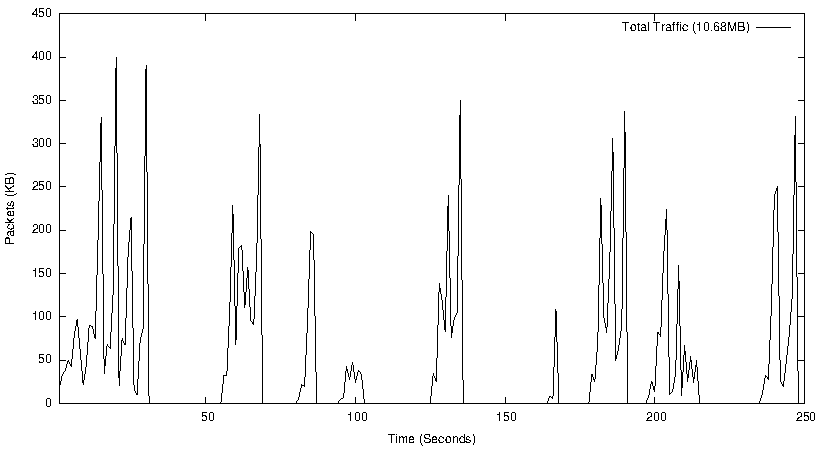
\includegraphics[scale=1.0]{jmdns10packet-distribution.pdf}
\caption{A JmDNS traffic histogram showing the Poisson-10 case.   } 
\label{indi:fig:jmdns-10-traffic}
\end{figure}
 

JmDNS on the other hand due of its design cannot meet the requested QoS limits.  The dynamics of the network and services is far too extreme for the conservative mDNS timer settings, designed solely for use on a LAN. Also, the extra redundancy in the messaging involved in an mDNS handshake, increases the latency too much to meet the required QoS. This is discussed in more detail in the next section to cohabit with the mDNS handshaking discussion and bandwidth requirements.   The more general issues of responsiveness are discussed in Section \ref{indi:sec:indepth}.

\subsection{Overhead Analysis}   
\label{subsec:overhead}

\begin{figure}
\centering
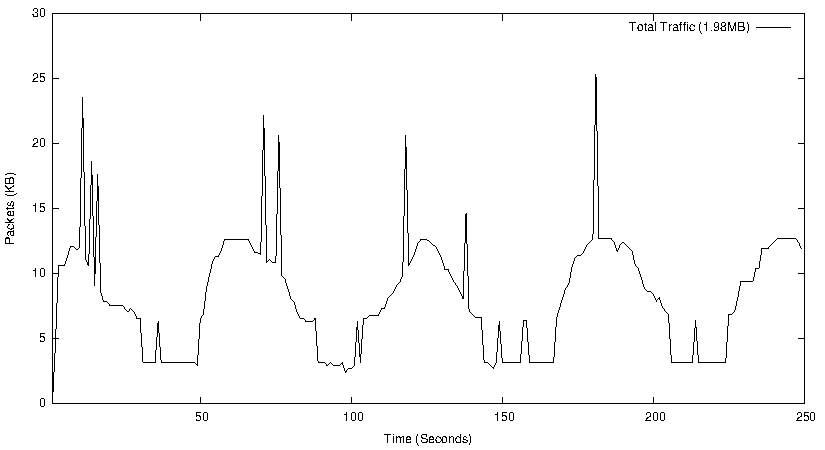
\includegraphics[scale=1.0]{indi20packet-distribution.pdf}
\caption{An INDI traffic histogram showing the Poisson-20 case.} 
\label{indi:fig:indi-20-traffic}
\end{figure}

At a high level, INDI and JmDNS operate in different modes.  INDI employs more of a proactive approach when addressing mobility whereas JmDNS has a defined sequence of message handshakes between JmDNS responders, which follow a combination of proactive and reactive solicitation.  However, in the JmDNS case, this interaction has a high short-term burst rate of several seconds and then a period of inactivity in transmitting messages across the network.  For INDI however, it proactively announces at a specific interval (1 second in these emulations) through the entire emulation. Therefore, although there are some minor peaks during service advertisement switch over in the INDI overhead histogram, this explains why is it is far more smooth overall.   Figures \ref{indi:fig:indi-10-traffic}, \ref{indi:fig:jmdns-10-traffic}, \ref{indi:fig:indi-20-traffic}, \ref{indi:fig:jmdns-20-traffic}, \ref{indi:fig:indi-30-traffic} and \ref{indi:fig:jmdns-30-traffic} show the traffic overhead caused by INDI and JmDNS for the three test cases covering Poisson mean intervals of 10, 20 and 30 seconds, respectively.

\begin{figure}
\centering
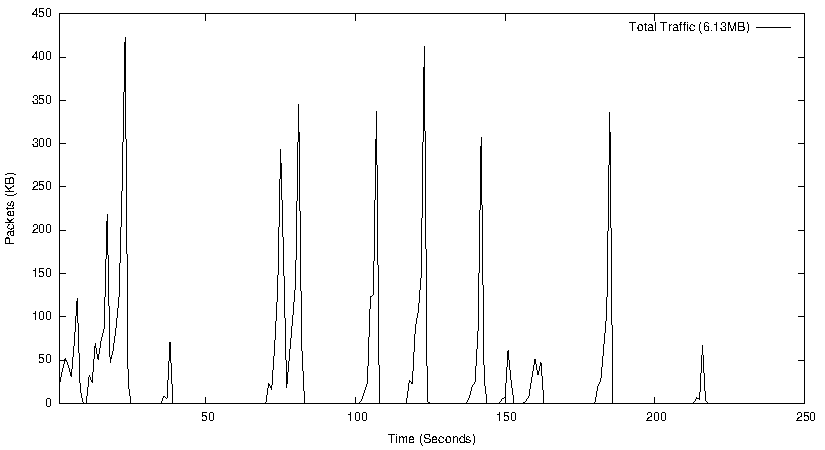
\includegraphics[scale=1.0]{jmdns20packet-distribution.pdf}
\caption{A JmDNS traffic histogram showing the Poisson-20 case.   } 
\label{indi:fig:jmdns-20-traffic}
\end{figure}

 Figures \ref{indi:fig:indi-10-traffic} and \ref{indi:fig:jmdns-10-traffic} show the traffic for the 10  second Poisson interval case.   It might seem clear from the proactive scheme that INDI sends out far more service advertisement requests with a shorter interval, creating consistent periodic traffic throughout the duration of the emulation. However, INDI messages are sent once and are not subjected to a number of handshakes with the client. In these experiments therefore, we can see that there are a lot less INDI messages and far less bandwidth consumed overall.  For each service advertisement request, JmDNS exchanges tens of message every time a service arrives onto the network and then remains quiet until the next advert comes onto the network.  This results in a far higher traffic burst rate and an accumulation of messages. Looking more closely at the scales in Figures \ref{indi:fig:indi-10-traffic} and \ref{indi:fig:jmdns-10-traffic}, we can in fact see that the JmDNS scale is one order of magnitude higher than that of INDI and hence, the total traffic consumed for INDI is 2.13 MB for the duration of the experiment, compared to 10.68MB for JmDNS. 
  
\begin{figure}[htb]
\centering
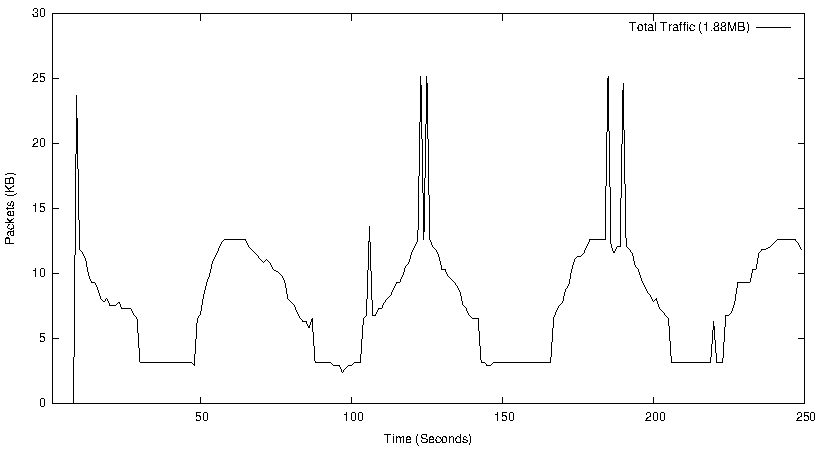
\includegraphics[scale=1.0]{indi30packet-distribution.pdf}
\caption{An INDI traffic histogram showing the Poisson-30 case.   } 
\label{indi:fig:indi-30-traffic}
\end{figure}

% change all to Poisson-10

 Considering the rather significant gains in success rates for INDI compared to JmDNS, it is somewhat surprising at first glance that JmDNS generates more traffic.  However, let's consider further evidence from our previous experiments \cite{Macker2011}.  In this experiment, we used Wireshark\footnote{http://www.wireshark.org/}, a sophisticated tool for capturing and parsing packets on the network, to observe the messages exchanged for a single service advertisement from INDI in Proactive mode and JmDNS, using a simple loopback network connector.  It was found that upon bootstrapping and discovering the first service on the network, a JmDNS node traverses through various stages e.g. server probing (three times), announcing (three two times) for resolving addresses and thereafter a further sequence for resolving services e.g. probers, announcers, and then type, service and service info resolvers.   This verbose activity results in 25 messages being exchanged between two JmDNS services to make the first discovery.  Thereafter, only the service sequence is followed but again this is several exchanges per service advertisement and thus causes large peaks at service interval times.  
 
The explanation for this extra bandwidth has already been discussed in Section \ref{sec:background}.  Since mDNS was designed to cover all LAN use cases, this is bound to have a knock on effect in terms of redundancy. Although a factor of 5 might at first glance seem high, mDNS attempts to deal with all combinations of clients and servers arriving at different times and is designed for an environment where services do not come onto the network very frequently.  Therefore, for example, over the course of several hours with one service arriving per hour (which is more in tune with the design requirements of mDNS), mDNS would indeed perform more efficiently than INDI set in proactive mode.  And although INDI could in theory be tuned to exhibit a similar behavior to mDNS by using a combination of proactive and reactive modes, it would unlikely to provide any benefit at all for use within a LAN.    So, the choice between the two for bandwidth efficiency depends completely on the dynamic nature of the services and the environment they are run in. Within a MANET however, the gains are clearly in the favor of INDI.   

\begin{figure}[htb]
\centering
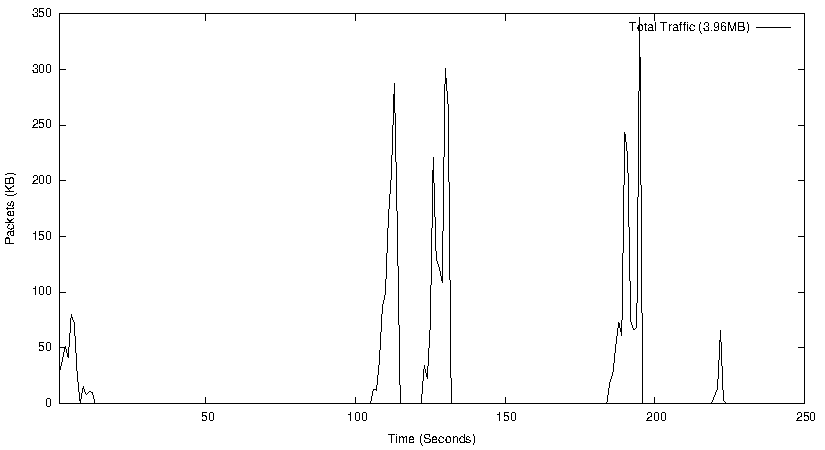
\includegraphics[scale=1.0]{jmdns30packet-distribution.pdf}
\caption{A JmDNS traffic histogram showing the Poisson-30 case.   } 
\label{indi:fig:jmdns-30-traffic}
\end{figure}

Figures \ref{indi:fig:indi-20-traffic}, \ref{indi:fig:jmdns-20-traffic}, \ref{indi:fig:indi-30-traffic} and \ref{indi:fig:jmdns-30-traffic} for Poisson-20 and Poisson-30 cases tell a similar story.  However, the results are not so extreme because there are less adverts being advertised during the course of the emulation.  For the 20 second interval, there are 15 service advertisements and for the 30 second interval, there are only 7. Therefore, the amount of traffic consumed is less for all cases.  The reductions in traffic for JmDNS are significant and depend directly on the number of advertisements. For example, whereas the JmDNS traffic for Poisson-10 was  10.68MB, Poisson-20 was 6.13 and Poisson-30 was 3.96, for INDI the traffic rates were 2.13, 1.98 and 1.88 MBs, respectively.  Even with 7 advertisements across the 250 second duration (less than two per minute), INDI still consumed less than half the traffic of JmDNS.  Further, as the result in table \ref{table:jmdns:comparison} shows, the success rates for INDI are more than twice that of JmDNS in these cases. For traffic therefore, there is little evidence from this study that the extra bandwidth consumed by JmDNS is having any effect of service discovery in this environment.  In the next section, we look at the the Poisson-10  and study the advert distribution and the reasons for the success differences between INDI and JmDNS more closely.


\subsection{A Closer Look at 10 Second Interval Case}   
\label{indi:sec:indepth}

\begin{figure}[htb]
\centering
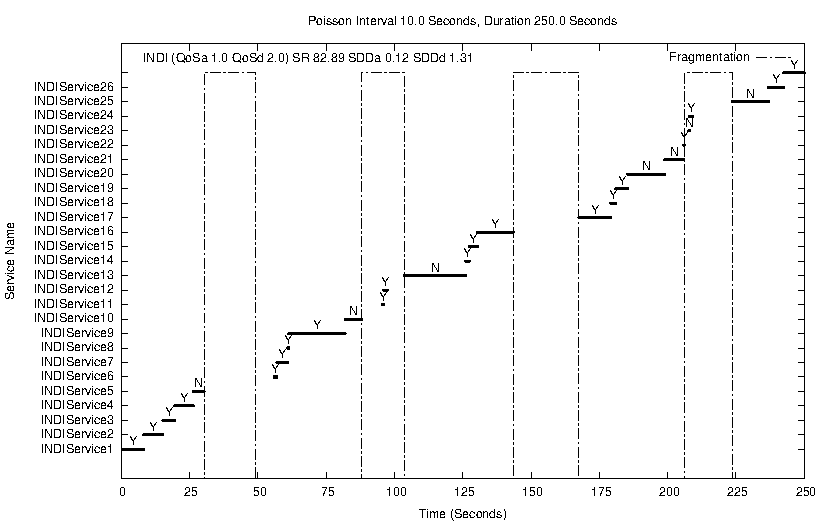
\includegraphics[scale=1.0]{indi10-1-2-results-distribution.pdf}
\caption{INDI: Shows the fragmentation pattern that affects the services' availability, the arrival and departure of each advert and the corresponding indication of successful detection of that advert (Y = success, N = failure).} 
\label{indi:fig:poisson-10-1-2}
\end{figure}

By observing the location and duration of the adverts during the course of the emulation for the Poisson-10 case, we discuss in this Section why certain adverts succeeded to be detected by a discovery systems and why others failed. Although we have 32 different cases in this category, we consider the two extreme cases here for illustration:

\begin{enumerate}
\item An  $SDD_{a}$ of 1 second and an $SDD_{d}$ 2 seconds.
\item An $SDD_{a}$ of 10 seconds and an $SDD_{d}$ of 20  seconds.
\end{enumerate}

In Figure \ref{indi:fig:poisson-10-1-2}, we show the performance of INDI when it has been requested to meet an $SDD_{a}$ of 1 second and an $SDD_{d}$ of 2 seconds. This plot shows a number of different things.   First, it overlays the connectivity diagram that representations the fragmentation in the network shown  in Figure \ref{indi:fig:emulationconnectivity}.  It then shows each service advertised during the course of the emulation (as per Figure \ref{indi:fig:poisson-10-adverts}) labelled by name on the y axis and annotated by a Y (success) or N (failure) if the service discovery system was able to detect that advert or not.   The services are also calibrated to show their visibility for consumers 5-9 after the fragmentation has been applied (as per Figure \ref{indi:fig:poisson-10-adverts-frag}). Finally, the statistics are provided about this run as a label at the top part of the graph, in the form:

\begin{verbatim}
INDI (QoSa 1.0 QoSd 2.0) SR 82.89 SDDa 0.12 SDDd 1.31
\end{verbatim}


\noindent which describe the parameters defined in Section \ref{sec:methodology}. This example shows that the INDI discovery system when applied to QoS parameters of $SDD_{a}$ of 1 second and $SDD_{d}$ of 2 seconds achieve as success rate (SR) of 82.89\%, an average service detection delay for arrival of 0.12 seconds and an average service detection delay for departure of 1.31 seconds.   

\begin{figure}[htb]
\centering
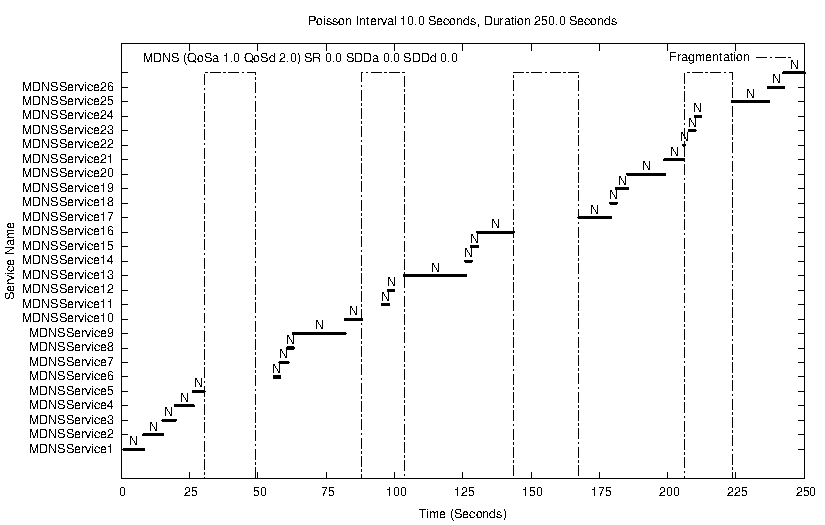
\includegraphics[scale=1.0]{jmdns10-1-2-results-distribution.pdf}
\caption{JmDNS: Successful service detection (Y = success, N = failure).} 
\label{jmdns:fig:poisson-10-1-2}
\end{figure}

Although INDI succeeds in detecting all of the services in the emulation, it cannot meet this QoS rate to the full. Looking in more detail at Figure \ref{indi:fig:poisson-10-1-2}, we can see that services around the fragmentations cause the most issues and since a success rate is applied to all consumers for each service, then the fragmented consumers are having a larger impact here.   The explanation for this affect is to do with the quantization of the proactive readvertisement interval and its alignment to services appearing and disappearing from the network.  Since INDI employed a proactive service announcement scheme (of rate 1 per second and a TTL of 2 seconds) for this experiment, these results are somewhat expected.   And upon further finer-grained analysis of the data, it was found in fact that an $SDD_{a}$ value of 1.8 and  an $SDD_{d}$ value of 2.7 is enough to achieve 100\% in all test cases for INDI covered in this study.  

The $SDD_{d}$ rate can be explained because when a service is deleted there is a slightly delay (100-200 ms) on the server whilst it starts the \emph{RecordReaper}  to detect the advert is expired.  During this time, it is possible in some case for the producer to proactively readvertise the service for a further TTL of 2 seconds.  And then on the service side,  since it takes 300-400 milliseconds to register a service in some cases, the range of 2.7 seconds can be expected in extreme circumstances.   

To combat these affects, INDI allows the tuning of both the proactive service announcement interval and the TTL for a service advertisement. Decreasing these values can improve responsiveness of the system, with the overhead of increased network bandwidth.  The decision for setting these values is application and network dependent. 

\begin{figure}[htb]
\centering
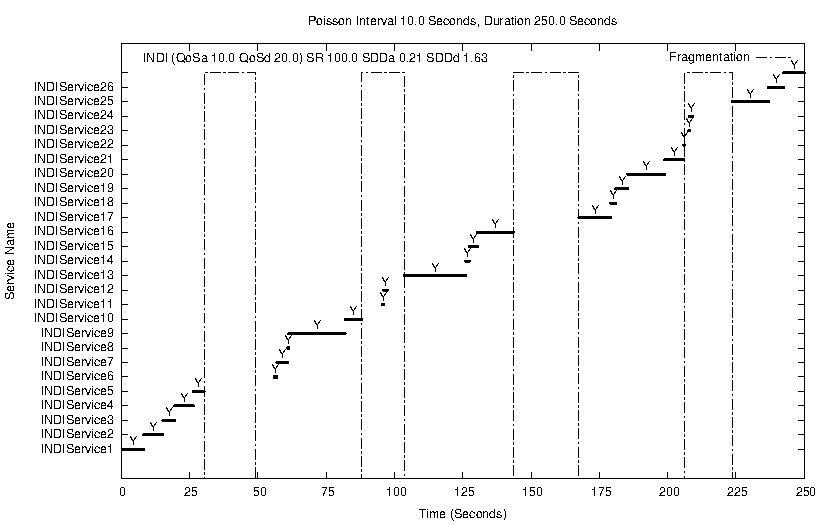
\includegraphics[scale=1.0]{indi10-10-20-results-distribution.pdf}
\caption{INDI: Successful service detection (Y = success, N = failure).} 
\label{indi:fig:poisson-10-10-20}
\end{figure}


In Figure \ref{jmdns:fig:poisson-10-1-2}, the story is quite different.  JmDNS was unable to discover any services using these values for the QoS metric. Not only does JmDNS suffer from a finite advertisement sequence (several seconds normally) and therefore misses a number of adverts that go out of range because of this, it also does not provide sufficient timely notification internally when success has been reached. Therefore, JmDNS needs far more time to respond successfully to service advertisements and therefore, it cannot meet the dynamics exhibited here and the level of QoS defined.  

This is explained again by the significantly different design priorities for mDNS when discovering services.  Rather than dealing with responsiveness, it performs multiple queries in order to ensure the discovery of the new longer lived services but also, it attempts to deal with maintaining the state of node IP addresses in case of conflicts.  This extra level of state maintenance creates an extra overhead on the network that introduces more traffic and a longer delay in the initial discovery. This is therefore not a failing of JmDNS but rather a mismatch of its intended purpose. However, it does stress the importance on the level of configurability for offering flexible modes and timers that INDI strives to achieve.

\begin{figure}[htb]
\centering
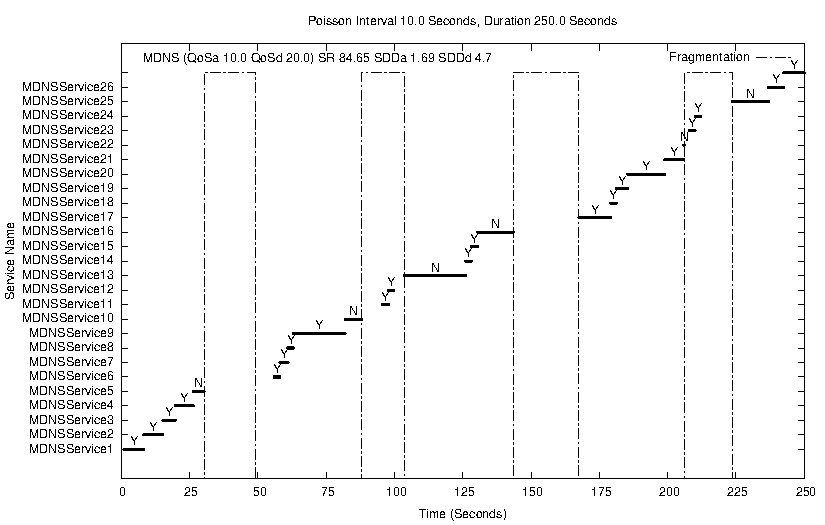
\includegraphics[scale=1.0]{jmdns10-10-20-results-distribution.pdf}
\caption{JmDNS: Successful service detection (Y = success, N = failure).} 
\label{jmdns:fig:poisson-10-10-20}
\end{figure}

The extended time period for $SDD_{a}$ of 10 seconds and $SDD_{d}$ of 20 seconds in Figure \ref{indi:fig:poisson-10-10-20} provides plenty of headroom for INDI to meet the expectations stated in the QoS. INDI achieves 100\% success with a delay of 0.21 seconds for the discovery of a service and an average of 1.63 seconds for the detection of a service when it departs from the network.

In Figure \ref{jmdns:fig:poisson-10-10-20} however, with a $SDD_{a}$ of 10 second and $SDD_{d}$ of 20 seconds, JmDNS  cannot achieve 100\%.  Its success rate is 84.65\% and it has a delay of 1.69 seconds for the discovery of a service (1.48 more than INDI) and an average of 4.7 seconds for the detection of a service (3.07 seconds more than INDI) when it departs from the network.

It is clear here, even with generous QoS constraints, that JmDNS suffers from the fragmentation of Consumers 5 to 9 when discovering services. It failed on \emph{MDNSService} services numbered 5, 10, 13, 16, 21 and 24.  All of these services either joined or left the network during the advertisement.  This can be explained by the follow reasons:

\begin{itemize}
\item \textbf{Services disappearing through fragmentation:} When a service is fragmented, mDNS has no mechanism for detecting this event. The TTL for an mDNS advert is 2 hours by default and since the producer does not know that consumers have gone out of range, it cannot notify them, and even if it did, there would be no connection.   Therefore, mDNS will always fail in this respect.  For INDI, it implements an adjustable TTL, which determines the rate at which adverts need to be refreshed and therefore it can detect absences.

\item \textbf{Services reappearing after fragmentation:} When a service reappears after a fragmentation, then mDNS can only discover it if it appears within its finite sequence of handshakes when a new service is advertised.  Therefore, MDNSService 17 was discovered by mDNS because it was advertised only a second or so before it came back into range and therefore within the normal mDNS handshaking sequence range.  Other advertisements could not be discovered because the interval was beyond its probing and announcement phases. 
\end{itemize}
 


\section{Conclusions}
\label{sec:conclusions}

In this \doctype, we have described the motivation, architecture, design, implementation and comparative analysis of INDI compared to an existing solutions for standardized service discovery on a local area network.   We have explained how  INDI achieves full interoperability with mDNS and that it offers attractive flexible service discovery profiles for optimization  in mobile networks. 

We have shown that INDI outperforms mDNS for a simple wireless networking mobile MANET scenario.  For bandwidth consumption, INDI achieved up to a six fold reduction in messages.  For success rates, even according to a modest quality of service metric for latencies of discovery and departure of services, INDI achieved at least a 17\% superior difference in results. It proved to be far more responsive and adaptable to network change.
 
Since the operating nature of INDI is peer-to-peer and therefore service providers advertise their own services, such gains make a significant difference. If INDI can provide more up-to-date service advertisements for exposing application endpoints, it follows therefore the connection to its endpoint to use the application is also likely to be more successful too.   This results in a far higher quality of experience for using services in a MANET environment in general.

Regarding future work we feel that INDI work could contribute in helping specify an open standard multi-hop multicast capable extension to mDNS and potentially other link local service discovery systems. Site-scoped multicast forwarding in mobile ad hoc networks is an example of where this could be applied in the short term.  Appropriate domains and rules need to be developed to make this both consistent and interoperable with mDNS and the DNS architecture.  Presently INDI provides a working prototype demonstrating that this type of design adaptation is achievable and beneficial.


\section*{Acknowledgments}

INDI work has been funded in part by the Office of Naval Research (ONR) Service Oriented Networks Operating in MANET (SONOMA) project.  Work in developing  mDNS interpoperability has been supported in part by the Groupwise Tactical Edge networking (GTEN) effort under �Networks Programs� within the Office of the Assistant Secretary of Defense (OASD), Research and Engineering. The authors wish like to thank Brian Adamson for his advice and SMF implementation used as an experimentation tool. We would also like to thank Andrew Harrison and Justin Dean for their work on the initial INDI implementation and experimentation efforts.  Finally, we would  like to thank the JmDNS team, and in particular, Pierre Frisch, who provided insight, guidance and exposed the timing interfaces for JmDNS tasks that made this work possible. 



\bibliographystyle{elsarticle-num}

\bibliography{fgcsbibs}

\end{document}

